\documentclass[table,aspectratio=169]{beamer}
%% Choose aspect ratio:
% [aspectratio=43]  % 4:3 (default)
% [aspectratio=169] % 16:9, wide

\usetheme[minimal, webfont, noheadline]{tugraz2018}
%\usetheme[iaik,]{tugraz2018}
%% Choose main theme variant:
% [standard]        % standard (default)
% [iaik]       % with institute's graphical acronym on the left
% [minimal]         % with reduced visuals

%% Choose your font style:
%                   % Helvetica (default for Corporate Design)
% [webfont]         % Source Sans Pro (as used on tugraz.at)
% [nofont]          % no font loaded - Computer Modern Sans

%% Choose your department's color instead of TU Graz red (optional):
% [arch]            % 
% [bau]             %
% [etit]            %
% [mbww]            %
% [tcvp]            %
% [mpug]            %
% [infbio]          %


\usepackage[utf8]{inputenc}
\usepackage[english]{babel}
%% Choose your language:
% [ngerman]   % German
% [english]   % English


%% Add your own packages, macros, etc.
\usepackage{xcolor,colortbl}
\usepackage{booktabs,nicematrix}
\usepackage{rotating}
\usepackage[style=alphabetic,backend=biber]{biblatex} % Bibliography
\addbibresource{\jobname.bib}                         % Bibliography
\usepackage{fontawesome}
\usepackage{filecontents}
\usepackage{setspace}
\usepackage{subcaption}
\usepackage{multirow}
\usepackage[linesnumbered,ruled,vlined]{algorithm2e}
\usepackage{algorithmicx}
\usepackage{algpseudocode}


\usetikzlibrary{calc,patterns,arrows.meta}
\usetikzlibrary{positioning}
\usetikzlibrary{cipher}
\setbeamersize
{
	text margin left=0.4cm,
	text margin right=0.4cm
}

%% Enter presentation metadata
\title{Improved Rectangle Attacks\\ on SKINNY and CRAFT}
\author{\textbf{Hosein Hadipour} \and Nasour Bagheri}
\date{FSE 2022 - Athens, Greece}
%\institute{IAIK}
\instituteurl{www.iaik.tugraz.at}

%% Logos
%\institutelogo{beamerthemetugraz/institute/IAIK}  % graphical acronym for [] theme (left margin)
% \additionallogo{figures/logo}  % additional institute/department logo (footline; optional)
% \logobar{Supported by: ...}  % sponsors (titlepage; optional)

%% Macros
\definecolor{gold}{HTML}{F0AB00}
\definecolor{bound}{HTML}{78b473}
\definecolor{best}{HTML}{e59352}
\definecolor{lin}{HTML}{285f82}
\definecolor{sub}{HTML}{78b473}
\definecolor{lightred}{rgb}{0.9, 0.2, 0.2}
\definecolor{lightblue}{rgb}{0, 0.5, 0.9}

\newcommand{\sparen}{\vspace*{-.3cm}}
\newcommand{\cipher}[1]{\textsc{#1}}

\newcolumntype{h}{>{\columncolor{bound}}r}
\newcolumntype{f}{>{\columncolor{best}}r}

\newcommand{\rightdownto}{\tikz{\draw[-{Latex[round,scale=1.2]}](0,0)-|(1.5ex,-1.5ex);}}
\newcommand{\doublearrowdown}{\tikz{\draw[-{Latex[round,scale=1.2]}](0,0)--(-1.5ex,-1.5ex);\draw[-{Latex[round,scale=1.2]}](0,0)--(1.5ex,-1.5ex);}}

\newcommand{\pattern}[2][64]{% #1 = bitsize, #2 = list of active bits
  \begin{tikzpicture}[x={(-0.2*0.75,0)},y={(0,0.3*0.75)}]
    \foreach \i in {#2} \fill (\i,0) rectangle (\i+1,1);
    \foreach \i in {1,2,...,#1} \draw[black!25] (\i,0) -- (\i,1);
    \foreach \i in {0,#1} \draw (\i,0) -- (\i,1);
    \foreach \i in {0,1} \draw (0,\i) -- (#1,\i);
  \end{tikzpicture}%
}
\newcommand{\patternGold}[2][64]{% #1 = bitsize, #2 = list of active bits
  \begin{tikzpicture}[x={(-0.2*0.75,0)},y={(0,0.3*0.75)}]
    \foreach \i in {#2} \fill[gold] (\i,0) rectangle (\i+1,1);
    \foreach \i in {1,2,...,#1} \draw[black!25] (\i,0) -- (\i,1);
    \foreach \i in {0,#1} \draw (\i,0) -- (\i,1);
    \foreach \i in {0,1} \draw (0,\i) -- (#1,\i);
  \end{tikzpicture}%
}

\newcommand{\mininecklace}[1][tug]{%
  \tikz[#1,thick,fill=white,baseline=0pt]{%
        \filldraw[fill=#1]    (0,0)  circle[radius=2pt];
        \filldraw[fill=white] (.2,0) circle[radius=2pt];
        \filldraw[fill=#1]    (.4,0) circle[radius=2pt];
        \filldraw[fill=white] (.6,0) circle[radius=2pt];
  }%
}

\makeatletter
\def\rowcolor{\noalign{\ifnum0=`}\fi\bmr@rowcolor}
\newcommand<>{\bmr@rowcolor}{%
    \alt#1%
        {\global\let\CT@do@color\CT@@do@color\@ifnextchar[\CT@rowa\CT@rowb}% 
        {\ifnum0=`{\fi}\@gooble@rowcolor}% 
}

\newcommand{\@gooble@rowcolor}[2][]{\@gooble@rowcolor@}
\newcommand{\@gooble@rowcolor@}[1][]{\@gooble@rowcolor@@}
\newcommand{\@gooble@rowcolor@@}[1][]{\ignorespaces}

\newcommand{\ddt}					{{\tt DDT}\xspace}
\newcommand{\bct}					{{\tt BCT}\xspace}
\newcommand{\dbt}					{{\tt UBCT}\xspace}
\newcommand{\bdt}					{{\tt LBCT}\xspace}
\newcommand{\dbct}					{{\tt DBCT}\xspace}
\makeatother

\begin{document}

\begin{frame}[plain]
  \maketitle
\end{frame}


\section*{}
\begin{frame}{Outline}
  \tableofcontents
\end{frame}

\section{Boomerang and Sandwich Distinguishers}
\sectionheader[\huge\color{tug}\faBook]{Boomerang and Sandwich Distinguishers}

\begin{frame}{Long Weak Differentials V.S. Two Short Strong Differentials}
\begin{figure}
\centering
\begin{tikzpicture}
\pgfmathsetmacro{\hstep}{0.7};
\pgfmathsetmacro{\vstep}{1.5};
\pgfmathsetmacro{\length}{8*\hstep};
\pgfmathsetmacro{\halflength}{\length/2};
\pgfmathsetmacro{\hight}{1};
\pgfmathsetmacro{\halfhight}{\hight/2};
\node[] (r1) at (0, 0) {$\Delta$};
\node[right=\hstep of r1] (c1) {};
\node[right=\halflength of c1] (c2) {};
\node[right=\halflength of c2] (c3) {};
\node[right=\hstep of c3] (c4) {$\nabla$};
\only<1->{%
\draw[rounded corners=3pt] ($(c1) + (0, -\halfhight)$) rectangle ($(c3) + (0, \halfhight)$) node[pos=.5] {$E:\mathbb{F}_{2}^{n} \rightarrow \mathbb{F}_{2}^{n}$};
\draw[->] (r1) -- (c1);
\draw[->] (c3) -- (c4);
\only<1>{%
\node[below=2*\halfhight of c2] (text) {$0 \lneq \Pr\{\Delta \xrightarrow{E} \nabla\} \lll 2^{-n}$};
}}
\only<2->{%
\draw[rounded corners=3pt, fill=white] ($(c1) + (0, -\halfhight)$) rectangle ($(c3) + (0, \halfhight)$);
\draw[gray] ($(c2) + (0, -\halfhight)$) -- ($(c2) + (0, \halfhight)$);
\node[] at ($0.5*(c1) + 0.5*(c2)$) {$E_{0}$};
\node[] at ($0.5*(c2) + 0.5*(c3)$) {$E_{1}$};
% Shift the axes down by \vstep units
\node[below=\vstep of r1] (r1) {$\Delta_{1}$};
\node[right=\hstep of r1] (c1) {};
\node[right=\halflength of c1] (c2) {};
\node[right=\halflength of c2] (c3) {};
\draw[rounded corners=3pt, fill=lightred] ($(c1) + (0, -\halfhight)$) rectangle ($(c2) + (0, \halfhight)$) node[pos=.5] {$E_{0}$};
\node[right=\hstep of c2] (temp) {$\Delta_{2}$};
\draw[->] (r1) -- (c1);
\draw[->] (c2) -- (temp);
\node[] at ($(c3) + (\hstep, 0)$) {$p = \Pr\{\Delta_{1} \xrightarrow{E_{0}} \Delta_{2}\}$};
% Shift the axes down by \vstep units
\node[below=\vstep of r1] (r1) {};
\node[right=\hstep of r1] (c1) {};
\node[right=\halflength of c1] (c2) {};
\node[right=\halflength of c2] (c3) {};
\draw[rounded corners=3pt, fill=lightblue] ($(c2) + (0, -\halfhight)$) rectangle ($(c3) + (0, \halfhight)$) node[pos=.5] {$E_{1}$};
\node[left=\hstep of c2] (temp1) {$\nabla_{2}$};
\node[right=\hstep of c3] (temp2) {$\nabla_{3}$};
\draw[->] (temp1) -- (c2);
\draw[->] (c3) -- (temp2);
\node[] at ($(c1) + (-\hstep, 0)$) {$q = \Pr\{\nabla_{2} \xrightarrow{E_{1}} \nabla_{3}\}$};
% Shift the axes down by \halfhight+0.2 units
\node[below=\halfhight+0.2 of r1] (r1) {};
\node[right=\hstep of r1] (c1) {};
\node[right=\halflength of c1] (c2) {};
\node[fill=gold] at (c2) {$p^{2}q^{2} \ggg 2^{-n}$}; 
}
\end{tikzpicture}
\end{figure}
\end{frame}

\begin{frame}{Combine Two Short Differentials in ACPC Setting \cite{fse_Wagner99}}
\begin{figure}[ht]
\centering
\begin{tikzpicture}[yscale=0.6,xscale=1, baseline=-1cm, thin]
\pgfmathsetmacro{\deltai}{2.4};
\pgfmathsetmacro{\nablao}{2.6};
\pgfmathsetmacro{\depth}{4.1};
\pgfmathsetmacro{\halfdepth}{\depth/2};
\pgfmathsetmacro{\quarterfdepth}{\depth/4};
\pgfmathsetmacro{\verticaldownshift}{1.2};
\node (p1) at (0, 0) {$p_{1}$};
\node (p2) at ($(p1) + (\deltai, -\verticaldownshift)$) {$p_{2}$};
\node[below=\halfdepth of p1] (x1) {$x_{1}$};
\node[below=\halfdepth of p2] (x2) {$x_{2}$};
\node[box, below=\quarterfdepth of p1.center, fill=lightred] (e0l1) {$E_{0}$};
\node[box, below=\quarterfdepth of p2.center, fill=lightred] (e0l2) {$E_{0}$};
\node[below=\halfdepth of x1] (c1) {$c_{1}$};
\node[below=\halfdepth of x2] (c2) {$c_{2}$};
\node[box, below=\quarterfdepth of x1.center, fill=lightblue] (e1l1) {$E_{1}$};
\node[box, below=\quarterfdepth of x2.center, fill=lightblue] (e1l2) {$E_{1}$};
\draw[<->, dashed, red] (p1) -- node[above] {$\Delta_{1}$} (p2);
\draw[<->, dashed, red] (x1) -- node[below] {$\Delta_{2}$} (x2);
\draw[->] (p1) -- (e0l1) -- (x1);
\node[left=0.5 of x1] (pnode) {$\textcolor{white}{\Pr\{p_{3} \oplus p_{4} = \Delta_{1}\} = p^{2} \times q^{2}}$};
\draw[->] (x1) -- (e1l1) -- (c1);
\draw[->] (p2) -- (e0l2) -- (x2);
\draw[->] (x2) -- (e1l2) -- (c2);
\node[right=\nablao of c1] (c3) {\textcolor{white}{$c_{3}$}};
\node[right=\nablao of c2] (c4) {\textcolor{white}{$c_{4}$}};
\only<1-3>{
\node[left=1 of e0l1] (pnode) {$\Pr\{\Delta_{1}\xrightarrow{E_{0}} \Delta_{2}\} = p$};
}
\only<2->{%
\node[right=\nablao of c1] (c3) {$c_{3}$};
\node[right=\nablao of c2] (c4) {$c_{4}$};
\draw[<->, dashed, blue] (c1) -- node[above] {$\nabla_{3}$} (c3);
\draw[<->, dashed, blue] (c2) -- node[above] {$\nabla_{3}$} (c4);
}
\only<3>{
\node[left=1 of e1l1] (pnode) {$\Pr\{\nabla_{2}\xrightarrow{E_{1}} \nabla_{3}\} = q$};
}
\only<3->{%
\node[left=0.5 of x1] (pnode) {$\textcolor{white}{\Pr\{p_{3} \oplus p_{4} = \Delta_{1}\} = p \times q^{2} \times p}$};
\node[right=\nablao of x1] (x3) {$x_{3}$};
\node[right=\nablao of x2] (x4) {$x_{4}$};
\node[box, below=\quarterfdepth of x3.center, fill=lightblue] (e1r1) {$E_{1}$};
\node[box, below=\quarterfdepth of x4.center, fill=lightblue] (e1r2) {$E_{1}$};
\draw[<->, dashed, blue] (x1) -- node[above] {$\nabla_{2}$} (x3);
\draw[<->, dashed, blue] (x2) -- node[below] {$\nabla_{2}$} (x4);
\draw[->] (c3) -- (e1r1) -- (x3);
\draw[->] (c4) -- (e1r2) -- (x4);
}
\only<4>{
\node[left=1 of x1] (pnode) {$\Pr\{p_{3} \oplus p_{4} = \Delta_{1}\} = p^{2} \times q^{2}$};
\node[right=\nablao of p1] (p3) {$p_{3}$};
\node[right=\nablao of p2] (p4) {$p_{4}$};
\node[box, below=\quarterfdepth of p3.center, fill=lightred] (e0r1) {$E_{0}$};
\node[box, below=\quarterfdepth of p4.center, fill=lightred] (e0r2) {$E_{0}$};
\draw[->] (x3) -- (e0r1) -- (p3);
\draw[->] (x4) -- (e0r2) -- (p4);

\draw[<->, dashed, red] (x3) -- node[above] {$\Delta_{2}$} (x4);
\draw[<->, dashed, red] (p3) -- node[above] {$\Delta_{1}$} (p4);
}
\end{tikzpicture}
\end{figure}
\end{frame}

\begin{frame}{Upper and Lower Parts are Not Independent in Practice!}
From the attacker's perspective:
\begin{itemize}
\item[\textcolor{tuggreen}{\faCheckCircle}] Dependency can have a {\color{tuggreen} \textbf{positive}} effect
\begin{itemize}
\item Feistel Switch \cite{fse_Wagner99}
\item Ladder Switch and S-box Switch \cite{conf_asiacrypt_BiryukovK09}
\end{itemize}
\item[\textcolor{gold}{\faWarning}] Dependency can have a {\color{red} \textbf{negative}} effect
\begin{itemize}
\item Inconsistency between the upper and lower trail \cite{journals_tit_Murphy11}
\end{itemize}
\end{itemize}
\end{frame}

\begin{frame}{Sandwich Distinguisher \cite{conf_crypto_DunkelmanKS10, journals_joc_DunkelmanKS14}}
\vspace{-0.5cm}
\begin{figure}
\only<1->{
\begin{subfigure}{0.5\textheight}
\centering
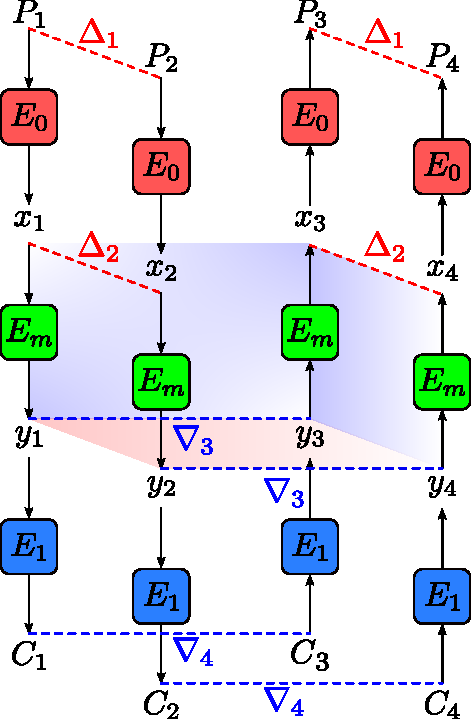
\includegraphics[width=0.85\textwidth]{./figures/sandwich.pdf}
\end{subfigure}
}
\only<1>{
$
\Pr(P_{3} \oplus P_{4} = \textcolor{red}{\Delta_{1}}) \approx p^{2}\times r \times q^{2}
$

\[r = r(\textcolor{red}{\Delta_{2}}, \textcolor{blue}{\nabla_{3}}) = \Pr\{E_{m}^{-1}(E_{m}(x) \oplus \textcolor{blue}{\nabla_{3}} ) \oplus E_{m}^{-1}(E_{m}(x \oplus \textcolor{red}{\Delta_{2}}) \oplus \textcolor{blue}{\nabla_{3}}) = \textcolor{red}{\Delta_{2}}\}\]
}
\only<2->{
\begin{subfigure}{0.6\textwidth}
\centering
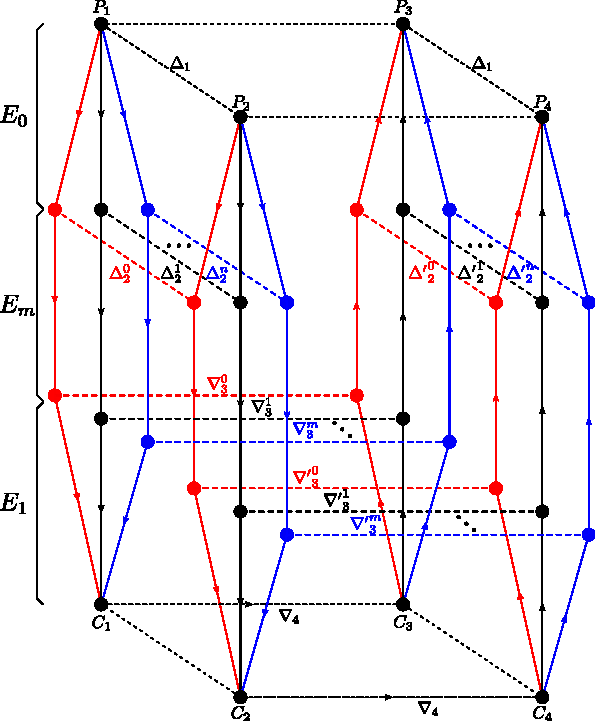
\includegraphics[width=0.5\textwidth]{./figures/sandwichcluster.pdf}
\end{subfigure}
{\scriptsize
\[
\Pr\left(P_{3} \oplus P_{4} = \Delta_{1}\right) = \sum_{\Delta_{2}, \Delta_{2}', \nabla_{3}, \nabla_{3}'} p_{\Delta_{2}}\times p_{\Delta_{2}'} \times r(\Delta_{2}, \Delta_{2}', \nabla_{3}, \nabla_{3}') \times q_{\nabla_{3}} \times q_{\nabla_{3}'} 
\]
}
}
\end{figure}
\end{frame}

\begin{frame}{Ladder Switch}
\vspace{-0.5cm}
\begin{figure}
\centering
\begin{tikzpicture}[yscale=0.6,xscale=1, baseline=-1cm, thin]
\onslide<1>{%
\pgfmathsetmacro{\deltai}{2.6};
\pgfmathsetmacro{\nablao}{2.8};
\pgfmathsetmacro{\depth}{5};
\pgfmathsetmacro{\halfdepth}{\depth/2};
\pgfmathsetmacro{\quarterfdepth}{\depth/4};
\pgfmathsetmacro{\verticaldownshift}{1.2};
\node (x1) at (0, 0) {$x_{1}$};
\node (x2) at ($(x1) + (\deltai, -\verticaldownshift)$) {$x_{2}$};
\node[below=\halfdepth of x1] (y1) {$y_{1}$};
\node[below=\halfdepth of x2] (y2) {$y_{2}$};
\node[box, below=\quarterfdepth of x1.center, fill=green] (e1l1) {$E_{m}$};
\node[box, below=\quarterfdepth of x2.center, fill=green] (e1l2) {$E_{m}$};
\draw[<->, dashed, red] (x1) -- node[above] {$\Delta_{2}$} (x2);
\draw[->] (x1) -- (e1l1) -- (y1);
\draw[->] (x2) -- (e1l2) -- (y2);
\node[right=\nablao of y1] (y3) {$y_{3}$};
\node[right=\nablao of y2] (y4) {$y_{4}$};
\draw[<->, dashed, blue] (y1) -- node[above] {$\nabla_{3}$} (y3);
\draw[<->, dashed, blue] (y2) -- node[above] {$\nabla_{3}$} (y4);
\node[right=\nablao of x1] (x3) {$x_{3}$};
\node[right=\nablao of x2] (x4) {$x_{4}$};
\node[box, below=\quarterfdepth of x3.center, fill=green] (e1r1) {$E_{m}$};
\node[box, below=\quarterfdepth of x4.center, fill=green] (e1r2) {$E_{m}$};
\draw[->] (y3) -- (e1r1) -- (x3);
\draw[->] (y4) -- (e1r2) -- (x4);
\draw[<->, red, dashed] (x3) -- node[above] {$\textcolor{red}{\Delta_{2}}$} (x4);
}
\only<2>{
\pgfmathsetmacro{\deltai}{0.1};
\pgfmathsetmacro{\nablao}{2.8};
\pgfmathsetmacro{\depth}{5};
\pgfmathsetmacro{\halfdepth}{\depth/2};
\pgfmathsetmacro{\quarterfdepth}{\depth/4};
\pgfmathsetmacro{\verticaldownshift}{0};
\node (x1) at (0, 0) {\textcolor{white}{$x_{1}$}};
\node (x2) at ($(x1) + (\deltai, -\verticaldownshift)$) {$x_{1} (= x_{2})$};
\node[below=\halfdepth of x1] (y1) {\textcolor{white}{$y_{1}$}};
\node[below=\halfdepth of x2] (y2) {$y_{1} = y_{2}$};
\node[box, below=\quarterfdepth of x1.center, fill=green] (e1l1) {$E_{m}$};
\node[box, below=\quarterfdepth of x2.center, fill=green] (e1l2) {$E_{m}$};
\draw[->] (x1) -- (e1l1) -- (y1);
\draw[->] (x2) -- (e1l2) -- (y2);

\node[right=\nablao of x1] (x1) {\textcolor{white}{$x_{1}$}};
\node (x2) at ($(x1) + (\deltai, -\verticaldownshift)$) {$x_{3} (= x_{4})$};
\node[below=\halfdepth of x1] (y3) {\textcolor{white}{$y_{1}$}};
\node[below=\halfdepth of x2] (y4) {$y_{3} = y_{4}$};
\node[box, below=\quarterfdepth of x1.center, fill=green] (e1l1) {$E_{m}$};
\node[box, below=\quarterfdepth of x2.center, fill=green] (e1l2) {$E_{m}$};
\draw[->] (y3) -- (e1l1) -- (x1);
\draw[->] (y4) -- (e1l2) -- (x2);
\draw[<->, dashed, blue] (y2.east) -- node[above] {$\nabla_{3}$} (y4.west);
}
\only<3>{
\pgfmathsetmacro{\deltai}{2.6};
\pgfmathsetmacro{\nablao}{0};
\pgfmathsetmacro{\depth}{5};
\pgfmathsetmacro{\halfdepth}{\depth/2};
\pgfmathsetmacro{\quarterfdepth}{\depth/4};
\pgfmathsetmacro{\verticaldownshift}{1.2};
\node (x1) at (0, 0) {};
\node (x2) at ($(x1) + (\deltai, -\verticaldownshift)$) {};
\node[] at (x1) {$x_{1} = (x_{3})$};
\node[] at (x2) {$x_{2} = (x_{4})$};
\node[below=\halfdepth of x1] (y1) {$y_{1} (= y_{3})$};
\node[below=\halfdepth of x2] (y2) {$y_{2} (= y_{4})$};
\node[box, below=\quarterfdepth of x1.center, fill=green] (e1l1) {$E_{m}$};
\node[box, below=\quarterfdepth of x2.center, fill=green] (e1l2) {$E_{m}$};
\draw[<->, dashed, red] (x1) -- node[above] {$\Delta_{2}$} (x2);
\draw[->] (x1) -- (e1l1) -- (y1);
\draw[->] (x2) -- (e1l2) -- (y2);
\node[right=\nablao of y1.center] (y3) {};
\node[right=\nablao of y2.center] (y4) {};
\node[right=\nablao of x1.center] (x3) {};
\node[right=\nablao of x2.center] (x4) {};
\node[box, below=\quarterfdepth of x1.east, fill=green] (e1r1) {$E_{m}$};
\node[box, below=\quarterfdepth of x2.east, fill=green] (e1r2) {$E_{m}$};
\draw[->] (y3) -- (e1r1) -- (x3);
\draw[->] (y4) -- (e1r2) -- (x4);

}
\end{tikzpicture}
\end{figure}
{\scriptsize 
\[r = r(\textcolor{red}{\Delta_{2}}, \textcolor{blue}{\nabla_{3}}) = \Pr\{E_{m}^{-1}(E_{m}(x) \oplus \textcolor{blue}{\nabla_{3}} ) \oplus E_{m}^{-1}(E_{m}(x \oplus \textcolor{red}{\Delta_{2}}) \oplus \textcolor{blue}{\nabla_{3}}) = \textcolor{red}{\Delta_{2}}\}\]
}
\pause
{\scriptsize
\[\textcolor{red}{\Delta_{2}} = 0 \Longrightarrow r = r(\textcolor{red}{0}, \textcolor{blue}{\nabla_{3}}) = 1\]
}
\pause
{\scriptsize
\[\textcolor{blue}{\nabla_{3}} = 0 \Longrightarrow r = r(\textcolor{red}{\Delta_{2}}, \textcolor{blue}{0}) = 1\]
}
\end{frame}

\begin{frame}{Effective Parameters in $p^{2}q^{2}r$ for SPN Ciphers}
\begin{itemize}
\item[\faCheckCircleO] $p$ is mostly determined by the number of active S-boxes in $E_{0}$
\item[\faCheckCircleO] $q$ is mostly determined by the number of active S-boxes in $E_{1}$
\item[\faCheckCircleO] $r$ is mostly determined by the number of \textcolor{red}{common} active S-boxes in $E_{m}$
\item[\faWarning] {\small Active S-boxes in $E_{0}, E_{1}$ are more expensive than common active S-boxes in $E_{m}$}
\end{itemize}
\begin{figure}
\centering
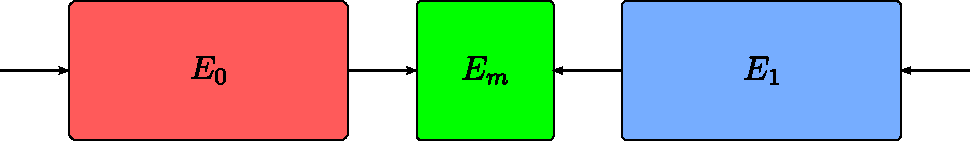
\includegraphics[width=0.65\textwidth]{./figures/milpdiff.pdf}
\end{figure}
\end{frame}

\section{Our Method To Find Sandwich Distinguishers}
\sectionheader[\huge\color{tug}\faCogs]{Our Method To Find Sandwich Distinguishers}

\begin{frame}{Our Method to Find Sandwich Distinguishers}
	Our method consists of 3 main steps:
	\begin{itemize}
		\pause
		\item[\faArrowCircleRight] Find the truncated upper and lower trails minimizing:
		\begin{itemize}
			\item number of active S-boxes in outer parts
			\item and number of common active S-boxes in the middle part
		\end{itemize}
		\pause
		\item[\faArrowCircleRight] Instantiate the discovered truncated trails with concrete differential trails
		\pause
		\item[\faArrowCircleRight] Compute $p$, $q$ and $r$ to derive the entire probability, i.e.,  $p^{2}q^{2}r$
	\end{itemize}
\end{frame}

\begin{frame}{Finding Appropriate Truncated Upper and Lower Trails}
	\begin{figure}
		\centering
		\begin{tikzpicture}[yscale=1,xscale=1,baseline=-0.6]
		%\node[] (top) at (0, 0) {top};
		%\node[] (bottom) at (0, -5) {bottom};
		\pgfmathsetmacro{\hstep}{2.7};
		\pgfmathsetmacro{\vstep}{1.2};
		\pgfmathsetmacro{\halfvstep}{\vstep/2};
		\pgfmathsetmacro{\quartervstep}{\vstep/4};
		\pgfmathsetmacro{\halfhstep}{\hstep/2};
		\pgfmathsetmacro{\quarterhstep}{\hstep/4};
		
		\only<1->{
			\node[] (c1) at (0, 0) {};
			\node[right=\hstep of c1] (c2) {};
			\node[right=\hstep of c2] (c3) {};
			\node[right=\hstep of c3] (c4) {};
			\node[] at ($0.5*(c2) + 0.5*(c3) + (0, -4*\vstep)$) {\scriptsize \textcolor{white}{$u_{i} - s_{i} \geq 0, ~~ l_{i} - s_{i} \geq 0, ~~ -u_{i} - l_{i} + s_{i} \geq -1.$}};
		}
		\only<1>{
			\draw[rounded corners=2pt] ($(c1) + (0, -\halfvstep)$) rectangle ($(c4) + (0, \halfvstep)$) node[pos=0.5] {$E$};
			\draw[<->, dashed, white] ($(c1) + (0, \halfvstep + 0.1)$) -- node[above] {$r_{0}$} ($(c2) + (0,
			\halfvstep + 0.1)$);
		}
		\only<2-5>{
			\draw[rounded corners=2pt] ($(c1) + (0, -\halfvstep)$) rectangle ($(c4) + (0, \halfvstep)$);
			\draw[] ($(c2) + (0, -\halfvstep)$) -- ($(c2) + (0, \halfvstep + 0.2)$);
			\draw[] ($(c3) + (0, -\halfvstep)$) -- ($(c3) + (0, \halfvstep + 0.2)$);
			\draw[<->, dashed] ($(c1) + (0, \halfvstep + 0.1)$) -- node[above] {$r_{0}$} ($(c2) + (0,
			\halfvstep + 0.1)$);
			\draw[<->, dashed] ($(c2) + (0, \halfvstep + 0.1)$) -- node[above] {$r_{m}$} ($(c3) + (0,
			\halfvstep + 0.1)$);
			\draw[<->, dashed] ($(c3) + (0, \halfvstep + 0.1)$) -- node[above] {$r_{1}$} ($(c4) + (0,
			\halfvstep + 0.1)$);
			\node[] (e0) at ($0.5*(c1) + 0.5*(c2)$) {$E_{0}$};
			\node[] (em) at ($0.5*(c2) + 0.5*(c3)$) {$E_{m}$};
			\node[] (e1) at ($0.5*(c3) + 0.5*(c4)$) {$E_{1}$};
		}
		\only<3-5>{%
			\node[below=\vstep of c1] (c1) {};
			\node[right=\hstep of c1] (c2) {};
			\node[right=\hstep of c2] (c3) {};
			\node[right=\hstep of c3] (c4) {};
			\draw[] ($(c2) + (0, -\halfvstep)$) -- ($(c2) + (0, \halfvstep)$);
			\draw[rounded corners=2pt] ($(c1) + (0, -\halfvstep)$) rectangle ($(c3) + (0, \halfvstep)$);
			
			\node[box, minimum size=8] at ($(c1) + (\quarterhstep, \quartervstep)$) {{\scriptsize $s$}};
			\node[box, minimum size=8, fill=lightred] at ($(c1) + (\quarterhstep, 0)$) {{\scriptsize $s$}};
			\node[box, minimum size=8] at ($(c1) + (\quarterhstep, -\quartervstep)$) {{\scriptsize $s$}};
			
			\node[box, minimum size=8, fill=lightred] at ($(c1.east) + (\halfhstep, \quartervstep)$) {{\scriptsize $s$}};
			\node[box, minimum size=8] at ($(c1.east) + (\halfhstep, 0)$) {{\scriptsize $s$}};
			\node[box, minimum size=8, fill=lightred] at ($(c1.east) + (\halfhstep, -\quartervstep)$) {{\scriptsize $s$}};
			
			\node[box, minimum size=8, fill] at ($(c2) + (-\quarterhstep, \quartervstep)$) {{\scriptsize $s$}};
			\node[box, minimum size=8, fill] at ($(c2) + (-\quarterhstep, 0)$) {{\scriptsize $s$}};
			\node[box, minimum size=8, fill=lightred] at ($(c2) + (-\quarterhstep, -\quartervstep)$) {{\scriptsize $s$}};
			
			\node[box, minimum size=8] at ($(c2) + (\quarterhstep, \quartervstep)$) {{\scriptsize $s$}};
			\node[box, minimum size=8] at ($(c2) + (\quarterhstep, 0)$) {{\scriptsize $s$}};
			\node[box, minimum size=8, fill=lightred] at ($(c2) + (\quarterhstep, -\quartervstep)$) {{\scriptsize $s$}};
			
			\node[box, minimum size=8] at ($(c2.east) + (\halfhstep, \quartervstep)$) {{\scriptsize $s$}};
			\node[box, minimum size=8, fill=lightred] at ($(c2.east) + (\halfhstep, 0)$) {{\scriptsize $s$}};
			\only<5>{
				\node[box, minimum size=8, fill=yellow] at ($(c2.east) + (\halfhstep, 0)$) {{\scriptsize $s$}};
			}
			\node[box, minimum size=8] at ($(c2.east) + (\halfhstep, -\quartervstep)$) {{\scriptsize $s$}};
			
			\node[box, minimum size=8, fill=lightred] at ($(c3) + (-\halfhstep + \quarterhstep, \quartervstep)$) {{\scriptsize $s$}};
			\node[box, minimum size=8, fill=lightred] at ($(c3) + (-\halfhstep + \quarterhstep, 0)$) {{\scriptsize $s$}};
			\node[box, minimum size=8] at ($(c3) + (-\halfhstep + \quarterhstep, -\quartervstep)$) {{\scriptsize $s$}};
		}
		\only<4-5>{
			\node[below=\vstep of c1] (c1) {};
			\node[right=\hstep of c1] (c2) {};
			\node[right=\hstep of c2] (c3) {};
			\node[right=\hstep of c3] (c4) {};
			\draw[] ($(c3) + (0, -\halfvstep)$) -- ($(c3) + (0, \halfvstep)$);
			\draw[rounded corners=2pt] ($(c2) + (0, -\halfvstep)$) rectangle ($(c4) + (0, \halfvstep)$);
			
			\node[box, minimum size=8, fill=lightblue] at ($(c2) + (\quarterhstep, \quartervstep)$) {{\scriptsize $s$}};
			\node[box, minimum size=8, fill=lightblue] at ($(c2) + (\quarterhstep, 0)$) {{\scriptsize $s$}};
			\node[box, minimum size=8] at ($(c2) + (\quarterhstep, -\quartervstep)$) {{\scriptsize $s$}};
			
			\node[box, minimum size=8] at ($(c2.east) + (\halfhstep, \quartervstep)$) {{\scriptsize $s$}};
			\node[box, minimum size=8, fill=lightblue] at ($(c2.east) + (\halfhstep, 0)$) {{\scriptsize $s$}};
			\only<5>{%
				\node[box, minimum size=8, fill=yellow] at ($(c2.east) + (\halfhstep, 0)$) {{\scriptsize $s$}};
			}
			\node[box, minimum size=8] at ($(c2.east) + (\halfhstep, -\quartervstep)$) {{\scriptsize $s$}};
			
			\node[box, minimum size=8] at ($(c3) + (-\quarterhstep, +\quartervstep)$) {{\scriptsize $s$}};
			\node[box, minimum size=8] at ($(c3) + (-\quarterhstep, 0)$) {{\scriptsize $s$}};
			\node[box, minimum size=8, fill=lightblue] at ($(c3) + (-\halfhstep + \quarterhstep, -\quartervstep)$) {{\scriptsize $s$}};
			
			\node[box, minimum size=8] at ($(c3) + (\quarterhstep, \quartervstep)$) {{\scriptsize $s$}};
			\node[box, minimum size=8] at ($(c3) + (\quarterhstep, 0)$) {{\scriptsize $s$}};
			\node[box, minimum size=8, fill=lightblue] at ($(c3) + (\quarterhstep, -\quartervstep)$) {{\scriptsize $s$}};	
			
			\node[box, minimum size=8, fill=lightblue] at ($(c3.east) + (\halfhstep, \quartervstep)$) {{\scriptsize $s$}};
			\node[box, minimum size=8] at ($(c3.east) + (\halfhstep, 0)$) {{\scriptsize $s$}};
			\node[box, minimum size=8, fill=lightblue] at ($(c3.east) + (\halfhstep, -\quartervstep)$) {{\scriptsize $s$}};
			
			\node[box, minimum size=8] at ($(c4) + (-\quarterhstep, +\quartervstep)$) {{\scriptsize $s$}};
			\node[box, minimum size=8] at ($(c4) + (-\quarterhstep, 0)$) {{\scriptsize $s$}};
			\node[box, minimum size=8, fill=lightblue] at ($(c4) + (-\quarterhstep, -\quartervstep)$) {{\scriptsize $s$}};
		}
		\only<5>{
			\node[] at ($0.5*(c2) + 0.5*(c3) + (0, -\vstep)$) {\scriptsize $\textcolor{red}{u_{i}} - s_{i} \geq 0, ~~ \textcolor{blue}{\ell_{i}} - s_{i} \geq 0, ~~ -\textcolor{red}{u_{i}} - \textcolor{blue}{\ell_{i}} + s_{i} \geq -1$};
		}
		
		
		%########################################
		\only<6->{
			\draw[rounded corners=2pt] ($(c1) + (0, -\halfvstep)$) rectangle ($(c4) + (0, \halfvstep)$);
			\draw[] ($(c2) + (0, -\halfvstep)$) -- ($(c2) + (0, \halfvstep + 0.2)$);
			\draw[] ($(c3) + (0, -\halfvstep)$) -- ($(c3) + (0, \halfvstep + 0.2)$);
			\draw[<->, dashed] ($(c1) + (0, \halfvstep + 0.1)$) -- node[above] {$r_{0}$} ($(c2) + (0,
			\halfvstep + 0.1)$);
			\draw[<->, dashed] ($(c2) + (0, \halfvstep + 0.1)$) -- node[above] {$r_{m}$} ($(c3) + (0,
			\halfvstep + 0.1)$);
			\draw[<->, dashed] ($(c3) + (0, \halfvstep + 0.1)$) -- node[above] {$r_{1}$} ($(c4) + (0,
			\halfvstep + 0.1)$);
			\node[] (e0) at ($0.5*(c1) + 0.5*(c2)$) {$E_{0}$};
			\node[] (em) at ($0.5*(c2) + 0.5*(c3)$) {$E_{m}$};
			\node[] (e1) at ($0.5*(c3) + 0.5*(c4)$) {$E_{1}$};
			\node[below=\vstep of c1] (c1) {};
			\node[right=\hstep of c1] (c2) {};
			\node[right=\hstep of c2] (c3) {};
			\node[right=\hstep of c3] (c4) {};
			\draw[] ($(c2) + (0, -\halfvstep)$) -- ($(c2) + (0, \halfvstep)$);
			\draw[rounded corners=2pt] ($(c1) + (0, -\halfvstep)$) rectangle ($(c3) + (0, \halfvstep)$);
			\node[] at ($0.5*(c1) + 0.5*(c2)$) (temp) {\footnotesize $\tilde{u}_{0}, \ldots, \tilde{u}_{k - 1}$};
			\node[] at ($0.5*(c2) + 0.5*(c3)$) (temp) {\footnotesize $u_{0}, \ldots, u_{t - 1}$};
			
			\node[below=\vstep of c1] (c1) {};
			\node[right=\hstep of c1] (c2) {};
			\node[right=\hstep of c2] (c3) {};
			\node[right=\hstep of c3] (c4) {};
			\draw[] ($(c3) + (0, -\halfvstep)$) -- ($(c3) + (0, \halfvstep)$);
			\draw[rounded corners=2pt] ($(c2) + (0, -\halfvstep)$) rectangle ($(c4) + (0, \halfvstep)$);
			\node[] at ($0.5*(c2) + 0.5*(c3)$) (temp) {\footnotesize $l_{0}, \ldots, l_{t - 1}$};
			\node[] at ($(c1.east) + (\halfhstep, +\halfvstep + 0.15)$) (w0) {\scriptsize $w_{0}$};
			\draw[<-, dashed] ($(c1) + (0, +\halfvstep + 0.15)$) -- (w0);
			\draw[->, dashed] (w0) -- ($(c2) + (0, +\halfvstep + 0.15)$);
			\node[] at ($(c2.east) + (\halfhstep, +\halfvstep + 0.15)$) (wm) {\scriptsize $w_{m}$};
			\draw[<-, dashed] ($(c2) + (0, +\halfvstep + 0.15)$) -- (wm);
			\draw[->, dashed] (wm) -- ($(c3) + (0, +\halfvstep + 0.15)$);
			\node[] at ($0.5*(c3) + 0.5*(c4)$) (temp) {\footnotesize $\tilde{l}_{0}, \ldots, \tilde{l}_{n - 1}$};
			\node[] at ($(c3.east) + (\halfhstep, +\halfvstep + 0.15)$) (w1) {\scriptsize $w_{1}$};
			\draw[<-, dashed] ($(c3) + (0, +\halfvstep + 0.15)$) -- (w1);
			\draw[->, dashed] (w1) -- ($(c4) + (0, +\halfvstep + 0.15)$);
			\node[] at ($0.5*(c2) + 0.5*(c3) + (0, -\vstep-\quartervstep + 0.4)$) {\footnotesize $\min  \sum_{i = 0}^{k - 1} w_{0}\cdot \tilde{u}_{i} + \sum_{j = 0}^{t - 1} w_{m}\cdot s_{j} + \sum_{k = 0}^{n - 1} w_{1}\cdot \tilde{l}_{k}.$};
			\node[] at ($0.5*(c2) + 0.5*(c3) + (0, -1.5*\vstep)$) {\footnotesize $u_{i} - s_{i} \geq 0, ~~ \ell_{i} - s_{i} \geq 0, ~~ -u_{i} - \ell_{i} + s_{i} \geq -1.$};
		}
		\end{tikzpicture}
	\end{figure}
\end{frame}

\begin{frame}{Instantiating Truncated Trails with Concrete Differentials}
	\begin{itemize}
		\pause
		\item[\faArrowCircleORight] We Instantiate the first and last parts with concrete bit-wise differentials
		\pause
		\item[\faArrowCircleORight] To compute $p$, $q$ and $r$ we fix the differences at only four positions
		\pause
		\item[\faWarning] \textbf{\textcolor{lightred}{Our distinguishers do \textbf{not} rely on differential characteristics for}} $E_{0}, E_{1}, E_{m}$
		%\item[\faCheckCircle] Compute $p^{2}q^{2}r$ based on differential effects $p, q$ and the $r$
	\end{itemize}
	\only<1-3>{%
		\begin{figure}
			\centering
			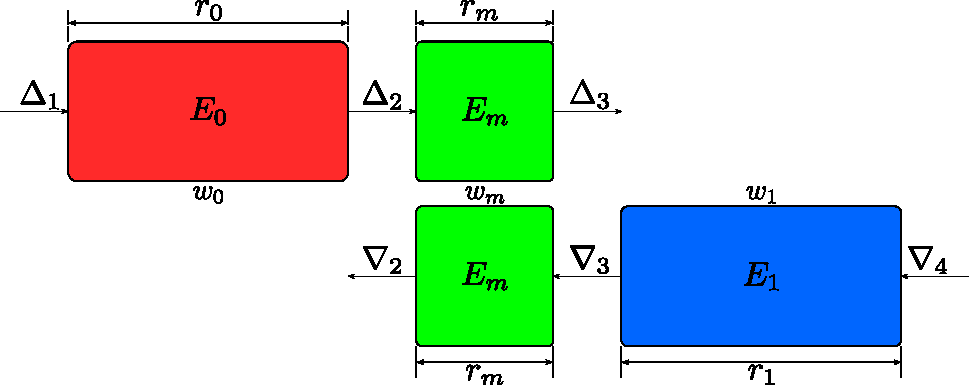
\includegraphics[width=0.55\textwidth]{./figures/milpdiff-1.pdf}
		\end{figure}
	}
	\only<4>{
		\begin{figure}
			\centering
			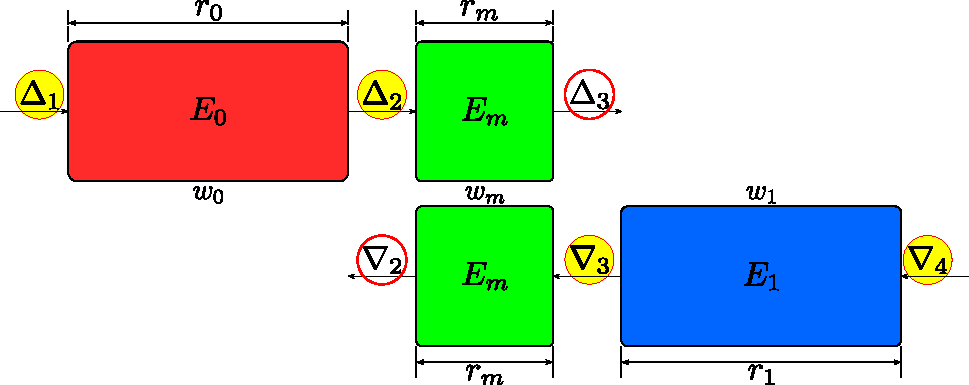
\includegraphics[width=0.55\textwidth]{./figures/milpdiff-2.pdf}
		\end{figure}
	}
\end{frame}

\section{BCT Framework and Our New Tools}
\sectionheader[\huge\color{tug}\faAlignJustify]{BCT Framework And Our New Tools}


\begin{frame}{BCT Framework}
\vspace{-0.5cm}
\begin{figure}
\centering
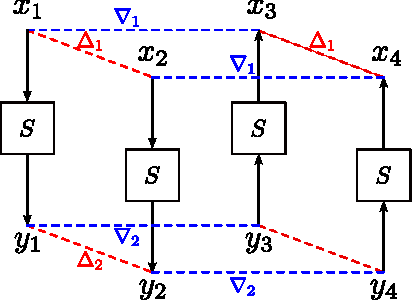
\includegraphics[height=0.3\textheight]{./figures/bct.pdf}
~~~~~~~~~~~~~~
\begin{tikzpicture}
\pgfmathsetmacro{\lth}{1.5};
\pgfmathsetmacro{\htt}{0.5};
\only<1>{
	\node[red] (d1) at (0, 0) {$\Delta_{1}$};
	\node[right=\lth of d1, red] (d2) {$\Delta_{2}$};
	\node[below=\htt of d1, blue] (n1) {$\nabla_{1}$};
	\node[right=\lth of n1, blue] (n2) {$\nabla_{2}$};
}
\only<2>{
	\node[red] (d1) at (0, 0) {$\Delta_{1}$};
	\node[right=\lth of d1, red] (d2) {$\Delta_{2}$};
	\node[below=\htt of d1, blue] (n1) {$\nabla_{1}$};
	\node[right=\lth of n1, blue] (n2) {$\nabla_{2}$};
	\draw[->] (d1) -- (d2);
	\draw[->] (n1) -- (n2);
}
\only<3>{
	\node[red] (d1) at (0, 0) {$\Delta_{1}$};
	\node[right=\lth of d1, gray] (d2) {$\Delta_{2}$};
	\node[below=\htt of d1, gray] (n1) {$\nabla_{1}$};
	\node[right=\lth of n1, blue] (n2) {$\nabla_{2}$};
	\draw[->] (d1) -- (n2);
}
\only<4>{
	\node[red] (d1) at (0, 0) {$\Delta_{1}$};
	\node[right=\lth of d1, red] (d2) {$\Delta_{2}$};
	\node[below=\htt of d1, gray] (n1) {$\nabla_{1}$};
	\node[right=\lth of n1, blue] (n2) {$\nabla_{2}$};
	\draw[->] (d1) -- (d2);
	\draw[->] (d1) -- (n2);
}
\only<5>{
	\node[red] (d1) at (0, 0) {$\Delta_{1}$};
	\node[right=\lth of d1, gray] (d2) {$\Delta_{2}$};
	\node[below=\htt of d1, blue] (n1) {$\nabla_{1}$};
	\node[right=\lth of n1, blue] (n2) {$\nabla_{2}$};
	\draw[->] (d1) -- (n2);
	\draw[->] (n1) -- (n2);
}
\only<6>{
	\node[red] (d1) at (0, 0) {$\Delta_{1}$};
	\node[right=\lth of d1, red] (d2) {$\Delta_{2}$};
	\node[below=\htt of d1, blue] (n1) {$\nabla_{1}$};
	\node[right=\lth of n1, blue] (n2) {$\nabla_{2}$};
	\draw[->] (d1) -- (d2);
	\draw[->] (d1) -- (n2);
	\draw[->] (n1) -- (n2);
}
\end{tikzpicture}
\end{figure}
\vspace{-0.4cm}
\begin{itemize}
\pause
\item[\faCheckCircle]{\scriptsize $\mathcal{X}_{\texttt{DDT}}(\Delta_{1}, \Delta_{2}) = \{x: S(x) \oplus S(x \oplus \Delta_{1}) = \Delta_{2}\}, \quad \texttt{DDT}(\Delta_{1}, \Delta_{2}) = \# \mathcal{X}_{\texttt{DDT}}(\Delta_{1}, \Delta_{2})$}
\pause
\item[\faCheckCircle]{\scriptsize $\mathcal{X}_{\texttt{BCT}}(\Delta_{1}, \nabla_{2}) = \{x: S^{-1}(S(x) \oplus \nabla_{2}) \oplus S^{-1}(S(x \oplus \Delta_{1}) \oplus \nabla_{2}) = \Delta_{1}\}, ~ \texttt{BCT}(\Delta_{1}, \nabla_{2}) = \# \mathcal{X}_{\texttt{BCT}}(\Delta_{1}, \nabla_{2})$ \hspace*{\fill} \cite{conf_eurocrypt_CidHPSS18}}
\pause
\item[\faCheckCircle]{\scriptsize $\texttt{UBCT}(\Delta_{1}, \Delta_{2}, \nabla_{2}) = \# \{x: x\in \mathcal{X}_{\texttt{BCT}}(\Delta_{1}, \nabla_{2}) \cap \mathcal{X}_{\texttt{DDT}}(\Delta_{1}, \Delta_{2})\}$ \hspace*{\fill} \cite{journals_tosc_WangP19}}
\pause
\item[\faCheckCircle]{\scriptsize $\texttt{LBCT}(\Delta_{1}, \nabla_{1}, \nabla_{2}) = \#\{x: x \in \mathcal{X}_{\texttt{BCT}}(\Delta_{1}, \nabla_{2}) \cap \mathcal{X}_{\texttt{DDT}}(\nabla_{1}, \nabla_{2})\}$ \hspace*{\fill} \cite{journals_tosc_SongQH19}}
%\pause
%\item[\faCheckCircle]{\scriptsize $\texttt{EBCT}(\Delta_{1}, \Delta_{2}, \nabla_{1}, \nabla_{2}) = \#\{x: x\in \mathcal{X}_{\texttt{BCT}}(\Delta_{1}, \nabla_{2}) \cap \mathcal{X}_{\texttt{DDT}}(\Delta_{1}, \Delta_{2}) \cap \mathcal{X}_{\texttt{DDT}}(\nabla_{1}, \nabla_{2})\}$ \hspace*{\fill} \cite{journals_tosc_BoukerrouHLMM20}}
\end{itemize}
\end{frame}

\begin{frame}{Double Boomerang Connectivity Table (\texttt{DBCT})}
\begin{figure}
\centering
\begin{tikzpicture}
\pgfmathsetmacro{\lth}{2};
\pgfmathsetmacro{\htt}{0.6};
\only<1>{
	\node[red] (d1) at (0, 0) {$\Delta_{1}$};
	\node[red] at ($(d1) + (\lth, 0)$) (d2) {$\Delta_{2}$};
	\node[blue] at ($(d1) + (\lth, -2*\htt)$) (n1) {$\bf{*}$};
	\node[blue] at ($(n1) + (\lth, 0)$) (n2) {$\nabla_{3}$};
	\draw[->] (d1) -- (d2);
	\draw[->] (n1) -- (n2);
	\draw[->] (d1) -- (n1);
	\draw[->] (d2) -- (n2);
}
\only<2>{
	\node[red] (d1) at (0, 0) {$\Delta_{1}$};
	\node[red] at ($(d1) + (\lth, 0)$) (d2) {$\bf{*}$};
	\node[blue] at ($(d1) + (\lth, -2*\htt)$) (n1) {$\nabla_{2}$};
	\node[blue] at ($(n1) + (\lth, 0)$) (n2) {$\nabla_{3}$};
	\draw[->] (d1) -- (d2);
	\draw[->] (n1) -- (n2);
	\draw[->] (d1) -- (n1);
	\draw[->] (d2) -- (n2);
}
\only<3>{
	\node[red] (d1) at (0, 0) {$\Delta_{1}$};
	\node[red] at ($(d1) + (\lth, 0)$) (d2) {$*$};
	\node[blue] at ($(d1) + (\lth, -2*\htt)$) (n1) {$*$};
	\node[blue] at ($(n1) + (\lth, 0)$) (n2) {$\nabla_{3}$};
	\draw[->] (d1) -- (d2);
	\draw[->] (n1) -- (n2);
	\draw[->] (d1) -- (n1);
	\draw[->] (d2) -- (n2);
}
\end{tikzpicture}
\end{figure}
\begin{itemize}
\item[\faCheckCircleO] {\scriptsize $\texttt{DBCT}^{\vdash}(\Delta_{1}, \Delta_{2}, \nabla_{3}) = \sum_{\nabla_{2}} \dbt(\Delta_{1}, \nabla_{2}, \Delta_{2})\cdot \bdt(\Delta_{2}, \nabla_{3}, \nabla_{2})$}
\pause
\item[\faCheckCircleO] {\scriptsize $\texttt{DBCT}^{\dashv}(\Delta_{1}, \nabla_{2}, \nabla_{3}) = \sum_{\Delta_{2}} \dbt(\Delta_{1}, \nabla_{2}, \Delta_{2})\cdot \bdt(\Delta_{2}, \nabla_{3}, \nabla_{2}).$}
\pause
\item[\faCheckCircleO] {\scriptsize $\texttt{DBCT}(\Delta_{1}, \nabla_{3}) = \sum_{\Delta_{2}}\dbct^{\vdash}(\Delta_{1}, \Delta_{2}, \nabla_{3}) = \sum_{\nabla_{2}}\dbct^{\dashv}(\Delta_{1}, \nabla_{2}, \nabla_{3}).$}
\end{itemize}
\end{frame}


\section{Application to CRAFT}
\sectionheader[\huge\color{tug}\faTh]{Application to CRAFT}

\begin{frame}{CRAFT \cite{journals_tosc_BeierleLMR19}}
\begin{figure}
\centering
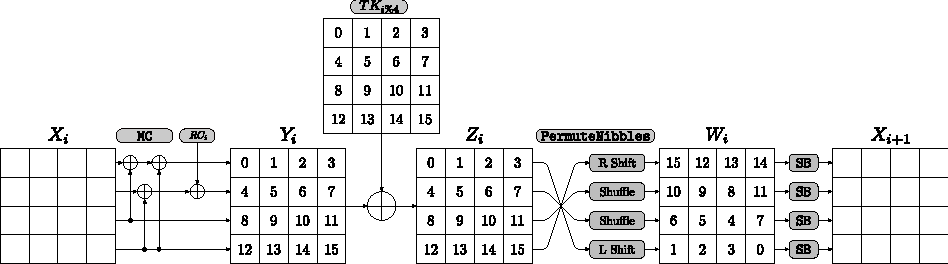
\includegraphics[width=0.9\textwidth]{./figures/craft_round_function.pdf}
\end{figure}
\end{frame}

\begin{frame}{A 6-round ST Deterministic Distinguisher for CRAFT}
\only<1>{%
\begin{figure}
\centering
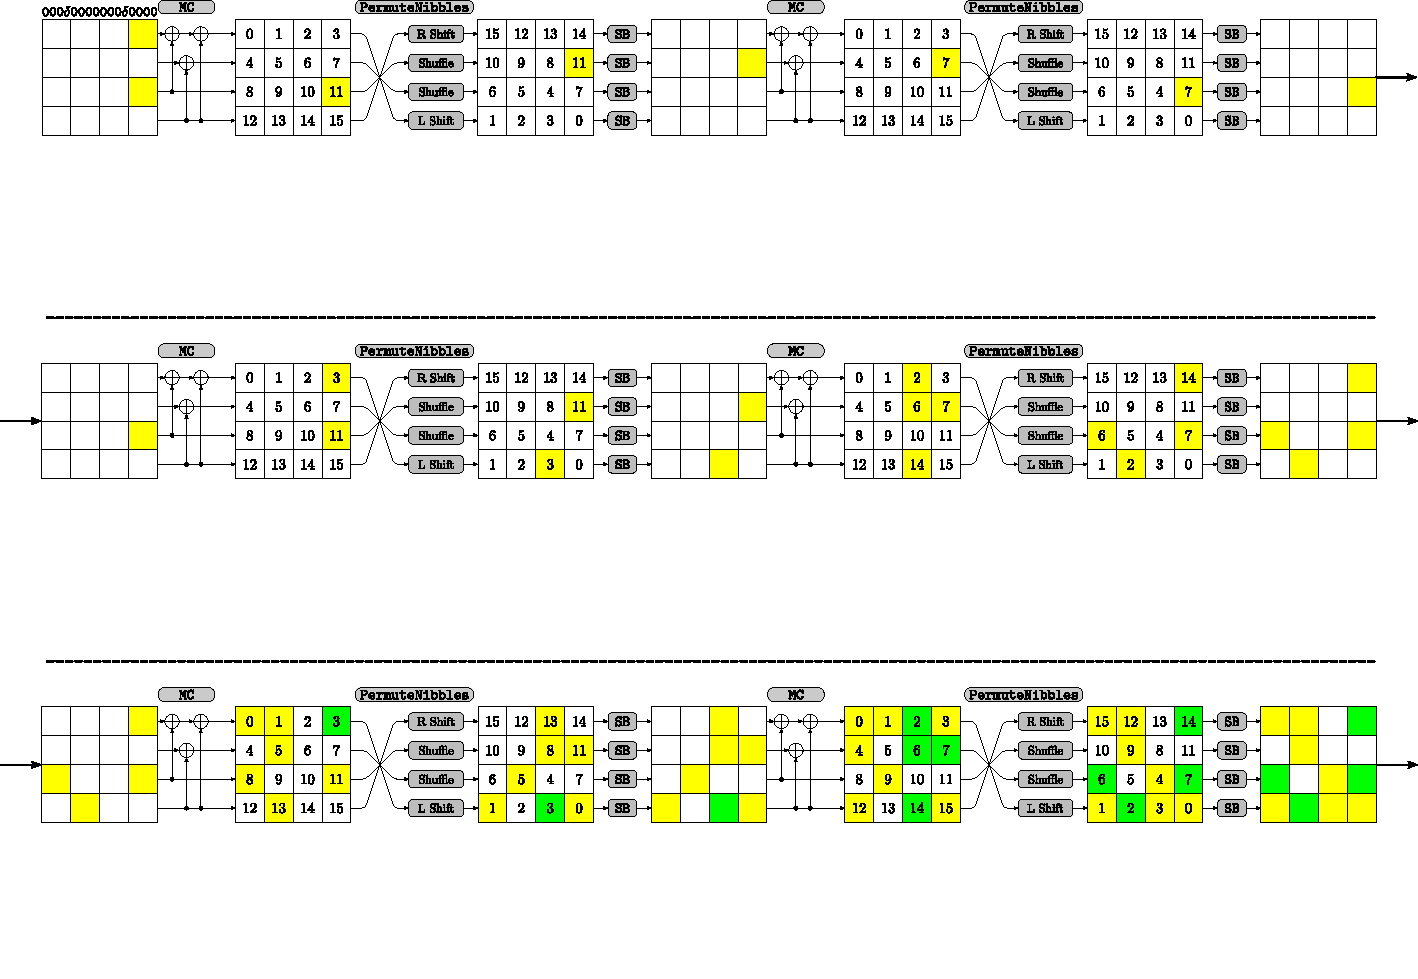
\includegraphics[width=0.55\textwidth]{./figures/boomerang_st_6r_three_stages_1.pdf}
\textcolor{white}{{\scriptsize $\Pr = 1$}}
\end{figure}
}
\only<2>{%
\begin{figure}
\centering
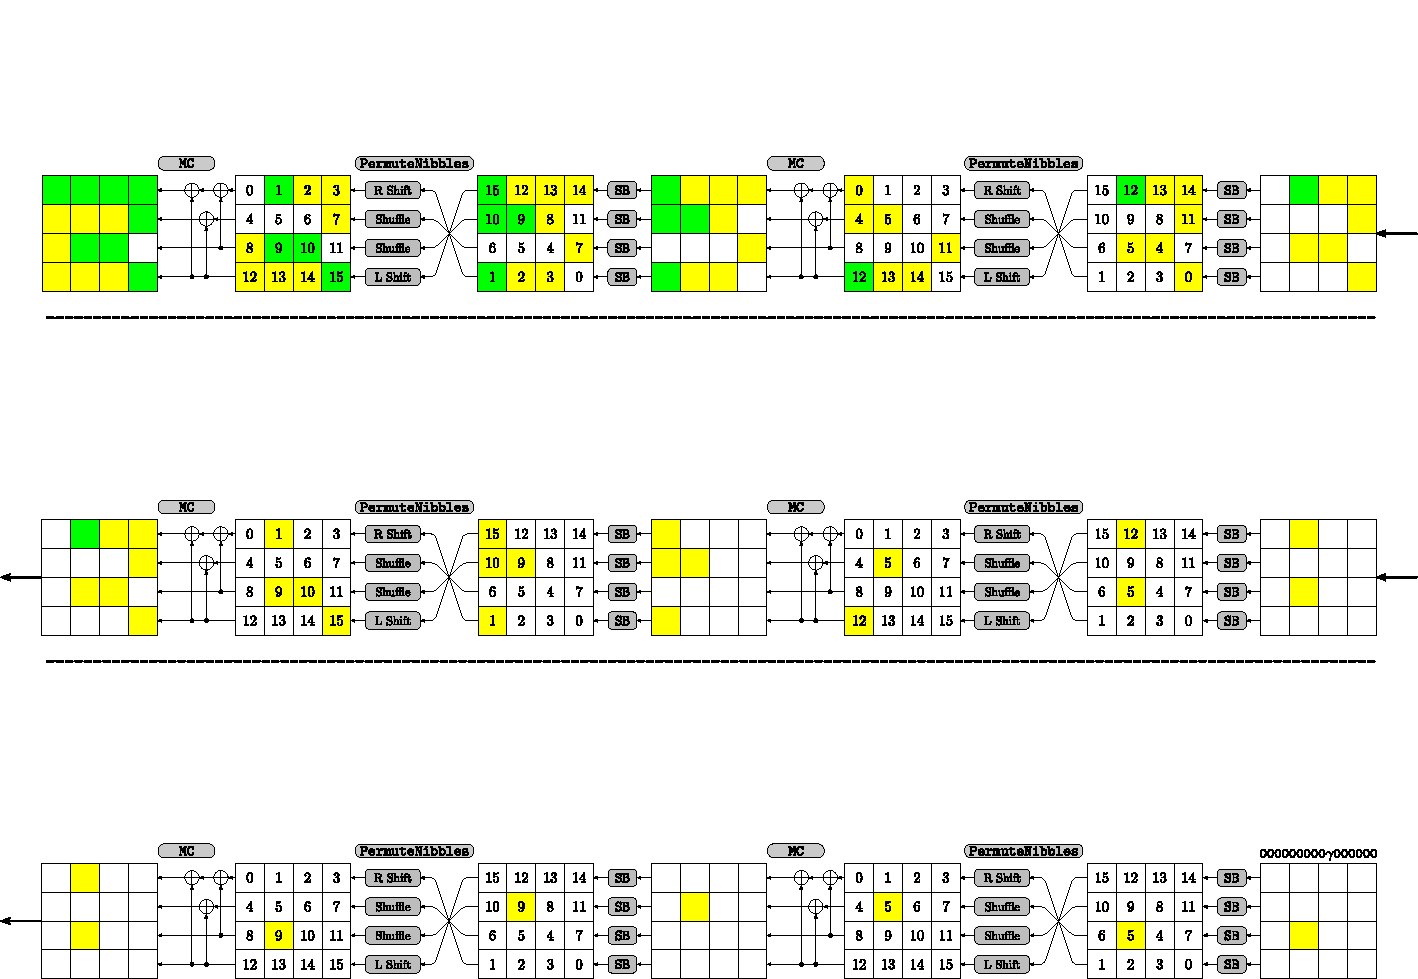
\includegraphics[width=0.55\textwidth]{./figures/boomerang_st_6r_three_stages_2.pdf}
\textcolor{white}{{\scriptsize $\Pr = 1$}}
\end{figure}	
}
\only<3>{%
	\begin{figure}
		\centering
		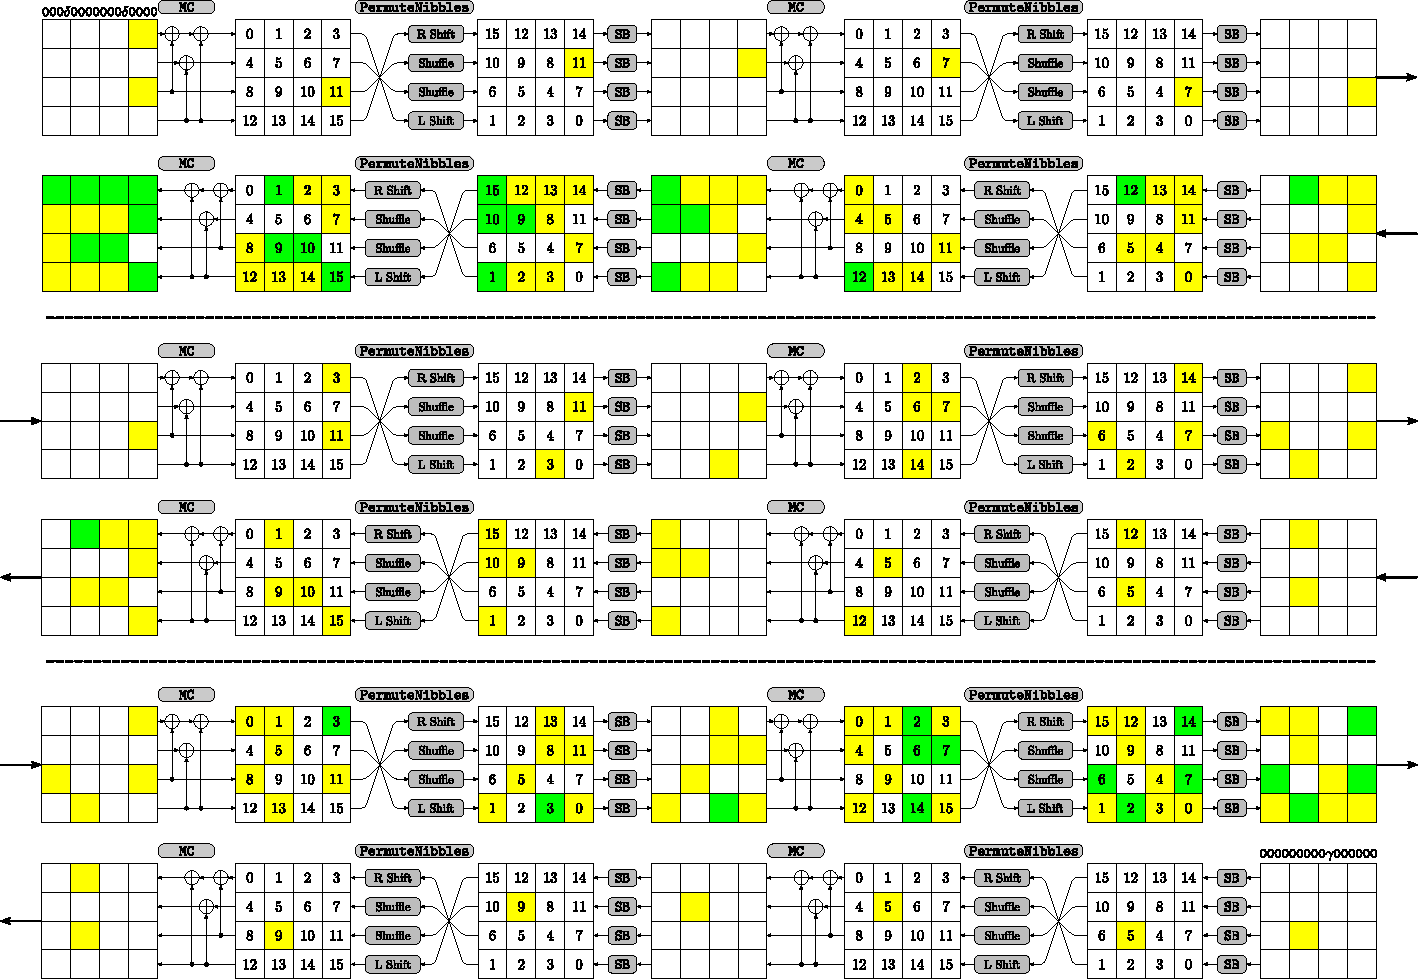
\includegraphics[width=0.55\textwidth]{./figures/boomerang_st_6r_three_stages_3.pdf}
		{\scriptsize $\Pr = 1$}
	\end{figure}	
}
\end{frame}

\begin{frame}{A 7-round Distinguisher (Extendable up to 14 rounds)}
\only<1>{%
\begin{figure}
\centering
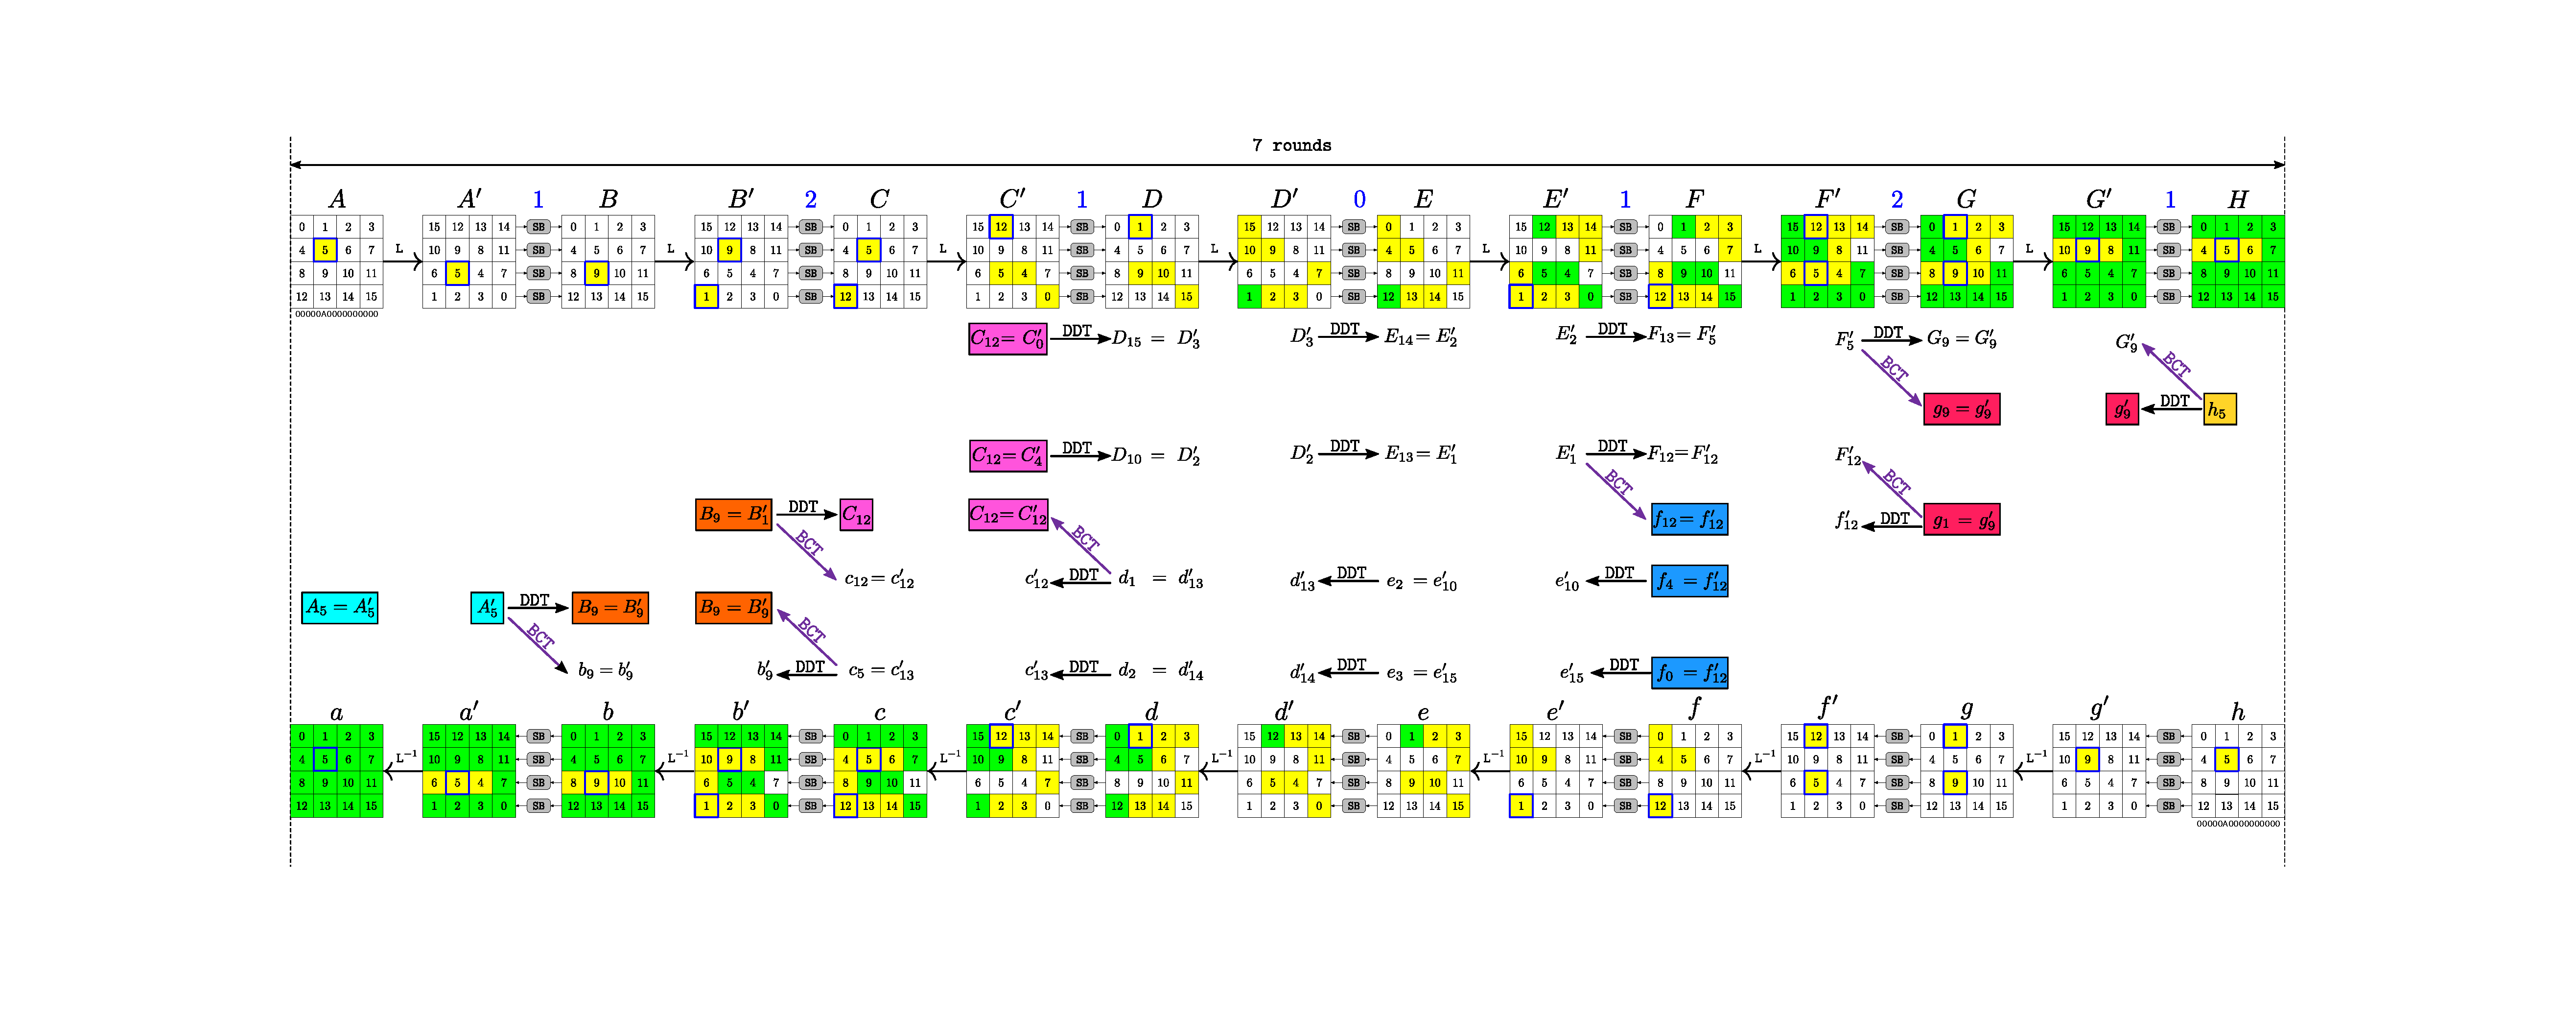
\includegraphics[width=\textwidth]{./figures/middle_part_7r_1.pdf}
\end{figure}
}
\only<2>{%
\begin{figure}
	\centering
	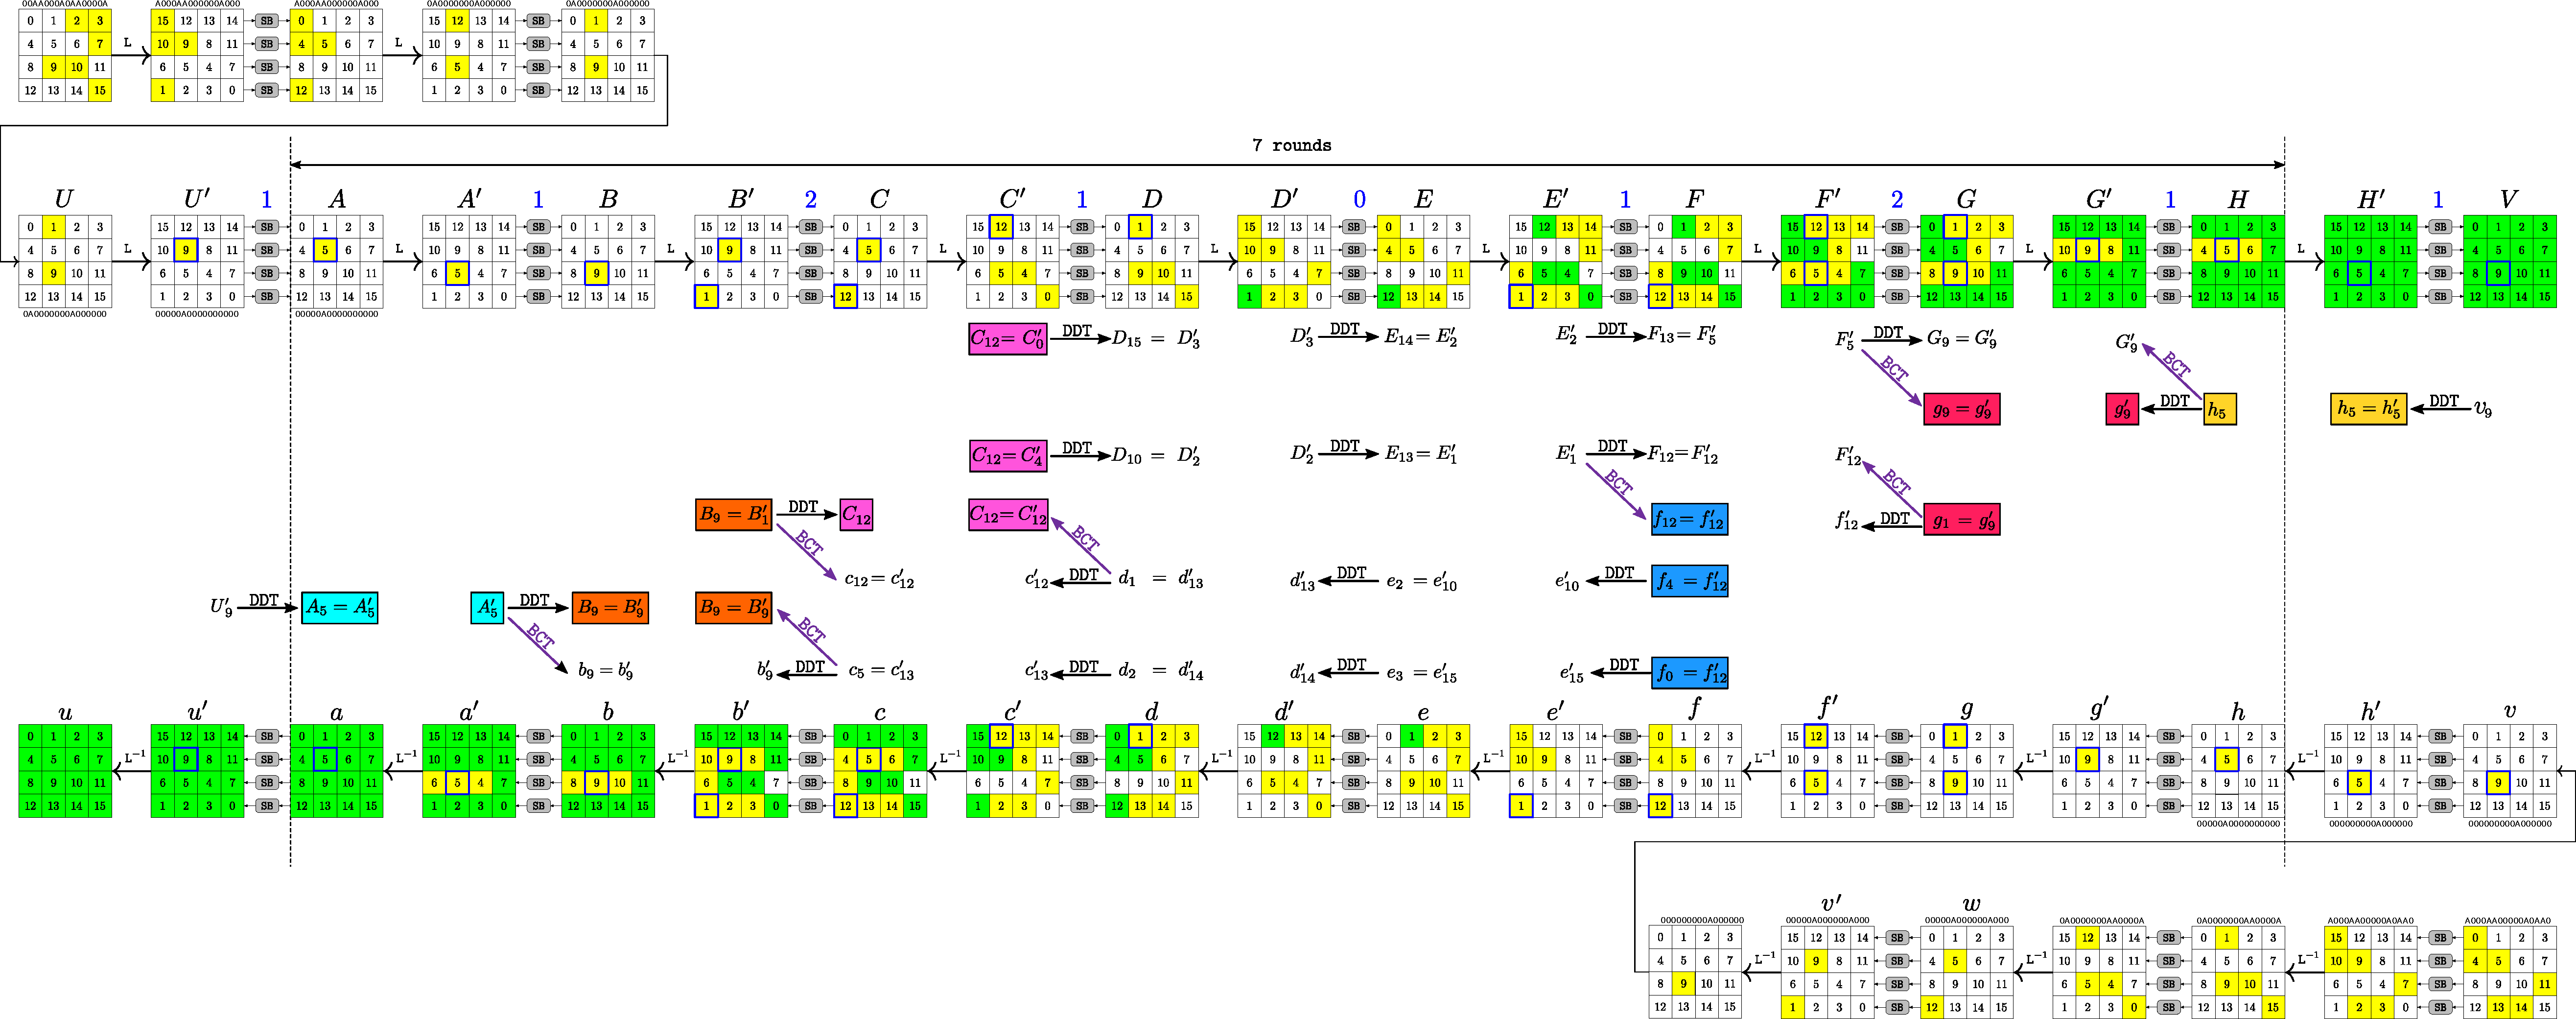
\includegraphics[width=\textwidth]{./figures/middle_part_7r_2.pdf}
\end{figure}
}
\only<3>{
\begin{figure}
\centering
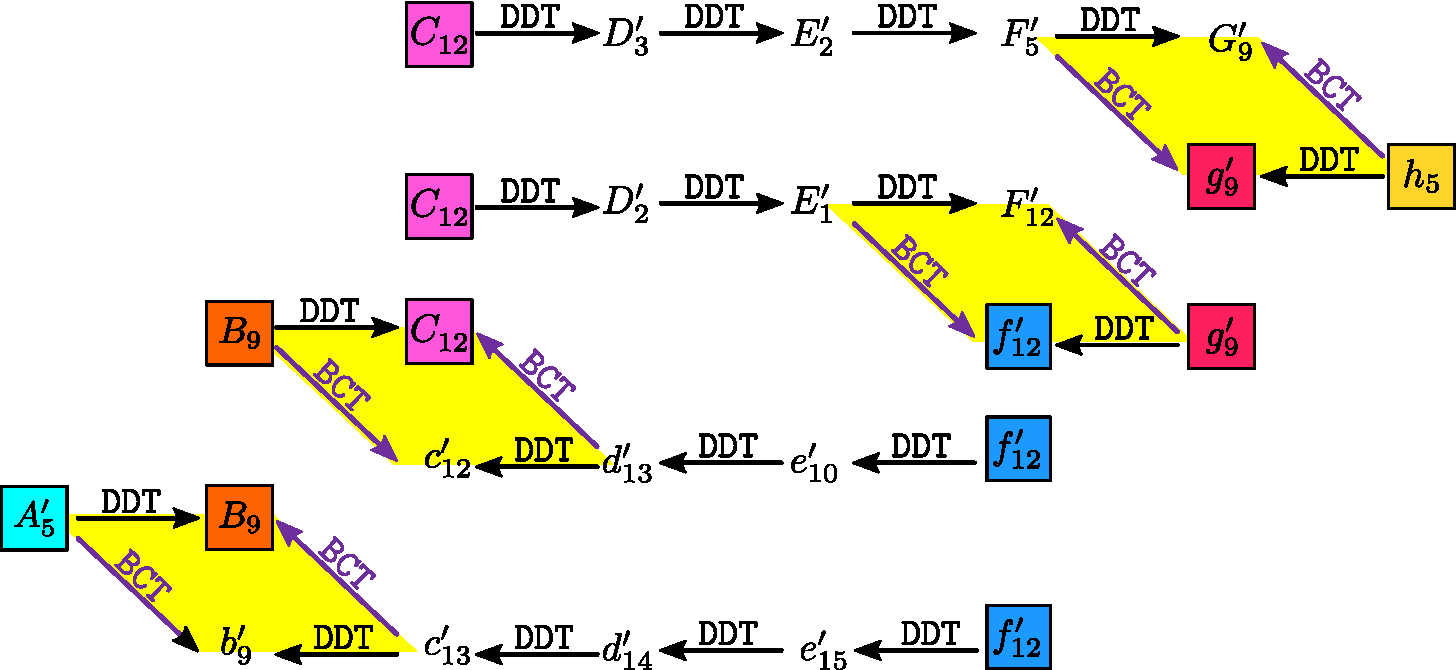
\includegraphics[width=0.55\textwidth]{./figures/middle_part_7r_3.pdf}
\end{figure}
\begin{center}
{\scriptsize $
\texttt{DBCT}_{\text{total}}= \texttt{DBCT}^{\vdash}(A_5, B_{9}, c_5)\cdot \texttt{DBCT}^{\vdash}(B_{9}, C_{12}, d_{1})\cdot\texttt{DBCT}^{\dashv}(E'_1, f'_{12}, g'_{9})
\cdot\texttt{DBCT}^{\dashv}(F'_5, g'_{9}, h_5)$}
{\scriptsize $
\text{Pr}_{\text{total}}= \Pr(d_{1} \xleftarrow{2 ~\ddt} f'_{12})\cdot
\Pr(c_{5} \xleftarrow{3 ~\ddt} f'_{12})\cdot \Pr(C_{12} \xrightarrow{2 ~\ddt} E'_1)\cdot
\Pr(C_{12} \xrightarrow{3 ~\ddt} F'_5)$ }
{\scriptsize
	$r = 2^{-8\cdot n}\cdot\sum_{B_{9}}\sum_{C_{12}}\sum_{g'_{9}}\sum_{f'_{12}}\sum_{c_5}\sum_{d_{1}} \sum_{E'_1}\sum_{F'_5} \dbct_{\text{total}}\cdot \text{Pr}_{\text{total}}$.
}
\end{center}
}
\end{frame}

\begin{frame}{Summary of Our Distinguishers for CRAFT}
	\begin{table}
		\centering
		\resizebox{0.5\textwidth}{!}{
			\begin{tabular}{c|c|c|c}
				\toprule
				Distinguisher Type & $\#$ Rounds & Probability & Reference\\ 
				\midrule
				\multirow{6}{*}{$ST$-$Differential$} & 9 & $2^{-40.20}$ &\multirow{6}{*}{\cite{journals_tosc_HadipourSNSB19}}\\
				& 10 & $2^{-44.89}$ & \\
				& 11 & $2^{-49.79}$ &\\
				& 12 & $2^{-54.48}$ &\\
				& 13 & $2^{-59.13}$ &\\
				& 14 & $2^{-63.80}$ &\\
				\midrule
				\multirow{8}{*}{$ST$-$Boomerang$} &	 6 & $\color{red}{\bf{1}}$ &\multirow{8}{*}{This Paper}\\
				& 7  & $\color{red}{\bf{2^{-4}}}$  &\\
				& 8  & $\color{red}{\bf{2^{-8}}}$  &\\
				& 9  & $\color{red}{\bf{2^{-14.76}}}$&\\
				& 10 & $\color{red}{\bf{2^{-19.83}}}$&\\
				& 11 & $\color{red}{\bf{2^{-24.90}}}$&\\
				& 12 & $\color{red}{\bf{2^{-34.89}}}$&\\
				& 13 & $2^{-44.89}$&\\
				& 14 & $2^{-55.85}$&\\
				\bottomrule   
			\end{tabular}
		}
	\end{table}
\end{frame}


\section{Application to SKINNY}
\sectionheader[\huge\color{tug}\faClipboard]{Application to SKINNY}

\begin{frame}{SKINNY \cite{conf_crypto_BeierleJKL0PSSS16}}
\begin{figure}
\centering
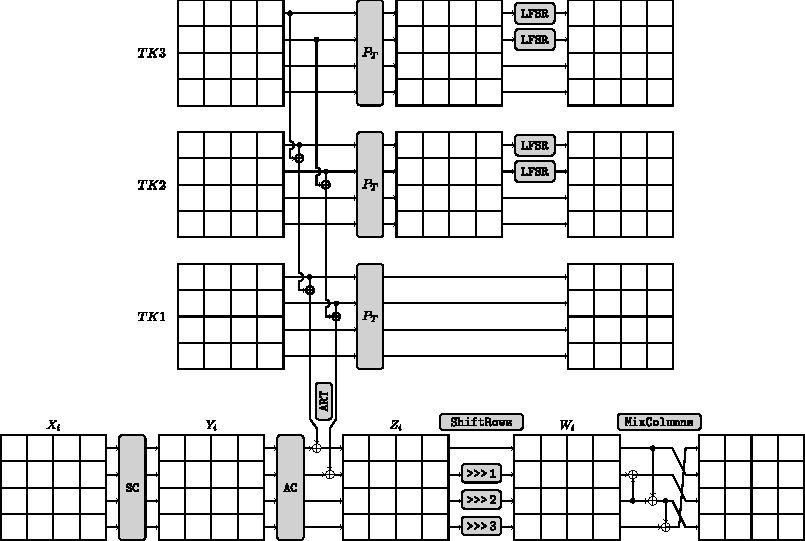
\includegraphics[width=0.6\textwidth]{./figures/skinny_round_function_complete.pdf}
\end{figure}
\end{frame}

\begin{frame}{18-round Practical Sandwich Distinguisher for SKINNY-128-256}
\centering
%\only<1>{%
%\begin{figure}
%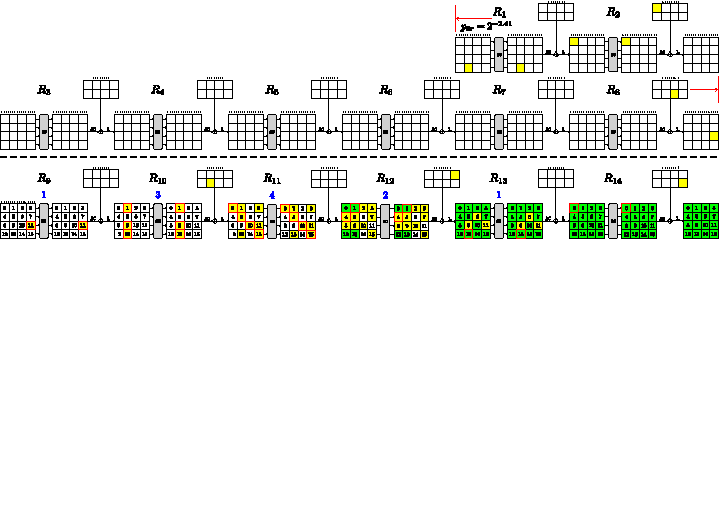
\includegraphics[width=0.57\textwidth]{./figures/rumi_64_192_bmd3_1.pdf}
%\end{figure}
%}
\only<1>{%
\begin{figure}
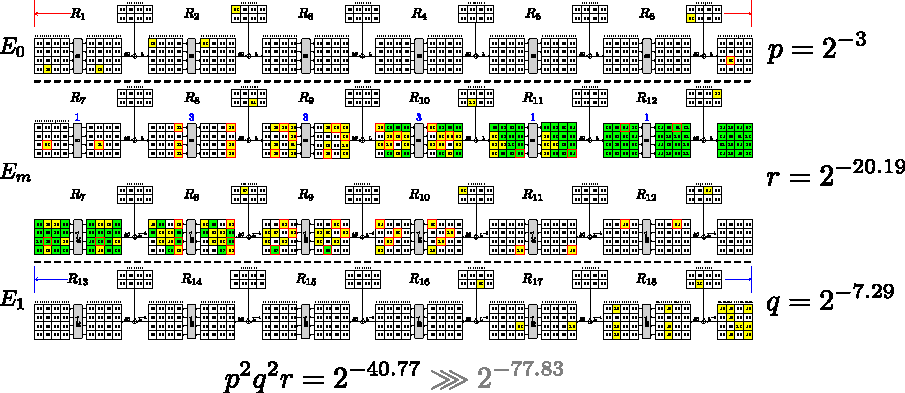
\includegraphics[width=.95\textwidth]{./figures/dufu_skinny_64_128_128_256.pdf}
\end{figure}
}
\end{frame}

\begin{frame}{Summary of Our Distinguishers for SKINNY}
	
	\begin{table}
		\centering
		\resizebox{0.5\textwidth}{!}{%
			\begin{tabular}{|c|c|c|c|c|}
				\toprule
				&  &  & \multicolumn{2}{c|}{Probability}\\
				\cline{4-5}
				Version & $n$ & $\#$Rounds & Our Distinguisher & 
				\cite{journals_tosc_SongQH19}\\
				\hline
				\hline
				\multirow{7}{*}{SKINNY-$n$-$2n$} & \multirow{3}{*}{64} & 17 &  $\textcolor{red}{\bf{2^{-26.54}}}$(\RN{2}) &  $2^{-29.78}$ \\
				%\cline{2-6}
				&  & 18 & $\textcolor{red}{\bf{2^{-37.90}}}$(\RN{2}) & $2^{-45.14}$ \\
				%\cline{2-6}
				&  & 19 & $\bf{2^{-51.08}}$(\RN{2}) & $2^{-65.62}$\\
				%\cline{2-6}
				\cline{2-5}			
				& \multirow{4}{*}{128} & 18 & $\textcolor{red}{\bf{2^{-40.77}}}$ (\RN{2}) & $2^{-77.83}$ \\
				%\cline{2-6}
				&  & 19 & $\bf{2^{-58.33}}$ (\RN{2}) & $2^{-97.53}$ \\
				%cline{2-6}
				&  & 20 & $\bf{2^{-85.31}}$ (\RN{1}) & $2^{-128.65}$ \\
				%\cline{2-6}
				&  & 21 & $\bf{2^{-114.07}}$ (\RN{2}) & $2^{-171.77}$ \\
				%\cline{2-6}
				\hline
				\multirow{6}{*}{SKINNY-$n$-$3n$} & \multirow{2}{*}{64} & 22 & $\textcolor{red}{\bf{2^{-38.84}}}$ (\RN{1}) & $2^{-42.98}$ \\
				&  & 23 & $\bf{2^{-52.84}}$ (\RN{1}) & $2^{-67.36}$ \\
				\cline{2-5}
				& \multirow{4}{*}{128} & 22 & $\textcolor{red}{\bf{2^{-40.57}}}$ (\RN{1})& $2^{-48.30}$ \\
				%\cline{2-6}
				&  & 23 & $\bf{2^{-56.47}}$ (\RN{1}) & $2^{-75.86}$\\
				%\cline{2-6}
				&  & 24 & $\bf{2^{-87.39}}$ (\RN{1}) & $2^{-107.86}$ \\
				%\cline{2-6}
				&  & 25 & $\bf{2^{-116.59}}$ (\RN{1}) & $2^{-141.66}$ \\
				%\cline{2-6}
				\bottomrule
			\end{tabular}
		}
	\end{table}
\end{frame}


\begin{frame}{Summary of Our Key Recovery Attacks}
	\begin{table}
		\centering
		\resizebox{0.9\textwidth}{!}{\begin{tabular}{|c|c|c|c|c|c|c|c|}
				\hline
				Scheme         &$\#$rounds &Data&Memory&Time & Attack &$P_s$ & Reference\\ \hline    
				SKINNY-64-128  &23/36 &$2^{60.54  }$&$2^{60.9 }$&$2^{120.7}$ &Rectangle  & 0.977&This paper\\ \hline 
				SKINNY-64-192 &29/40 &$2^{61.42 }$&$2^{80}$ &$2^{178}$&Rectangle& 0.977&This paper\\ \hline 
				SKINNY-128-256 &24/48 &$2^{125.21}$&$2^{125.54}$&$2^{209.85}$&Rectangle& 0.977&This paper\\ \hline 
				SKINNY-128-384  &30/56 &$2^{125.29}$&$2^{125.8}$ &$2^{361.68}$&Rectangle& 0.977&This paper\\ \hline 
				CRAFT &18/32 &$2^{60.92}$ &$2^{84}$ &$2^{101.7}$&Rectangle& 0.977&This paper\\  \hline   \hline
				
				SKINNY-64-128  &23/36 &$2^{62.47  }$&$2^{124 }$&$2^{125.91}$ &Impossible  & 1 &\cite{Liu_Ghosh_Song_2017}\\ \hline 
				SKINNY-64-192 &27/40 &$2^{63.5 }$&$2^{80}$ &$2^{165.5}$&Rectangle& 0.916&\cite{Liu_Ghosh_Song_2017}\\ \hline 
				SKINNY-128-256 &23/48 &$2^{124.47}$&$2^{248}$&$2^{251.47}$&Impossible& 1&\cite{Liu_Ghosh_Song_2017}\\ \hline 
				SKINNY-128-384  &28/56 &$2^{122}$&$2^{122.32}$ &$2^{315.25}$&Rectangle& 0.8315&\cite{zhao2020generalized}\\ \hline 
		\end{tabular}}
	\end{table}
\end{frame}

\section{Conclusion}
\sectionheader[\huge\color{tug}\faClockO]{Conclusion}

\begin{frame}{Our Main Contributions}
\begin{itemize}
\item[\faCheckCircleO] We introduced a heuristic method to search for sandwich distinguishers
\item[\faCheckCircleO] We introduced new tools in BCT framework (\texttt{DBCT}, ...)
\item[\faCheckCircleO] We significantly improved the rectangle attacks on SKINNY and CRAFT
\end{itemize}

\begin{center}
\vspace{0.5cm}

{\large Thanks for your attention!}

\vspace{0.5cm}
\url{https://github.com/hadipourh/Boomerang}
\end{center}
\end{frame}

















%%%%%%%%%%%%%%%%%%%%%%%%%%%%%%%%%%%%%%%%%%%%%%%%%%%%%%%%%%%%%%%%%%%%%%%%%%%%

\begin{frame}[allowframebreaks]{Bibliography}
  \printbibliography
\end{frame}

\begin{filecontents*}[overwrite]{\jobname.bib}

@misc{nist,
  author    = {{National Institute of Standards and Technology}},
  title     = {Submission Requirements and Evaluation Criteria for the Lightweight Cryptography Standardization Process},
  url       = {https://csrc.nist.gov/CSRC/media/Projects/Lightweight-Cryptography/documents/final-lwc-submission-requirements-august2018.pdf},
  year = {2018},
}

@article{xoodyak,
  author    = {Joan Daemen and
               Seth Hoffert and
               Micha{\"{e}}l Peeters and
               Gilles Van Assche and
               Ronny Van Keer},
  title     = {Xoodyak, a lightweight cryptographic scheme},
  journal   = {{IACR} Trans. Symmetric Cryptol.},
  volume    = {2020},
  number    = {{S1}},
  pages     = {60--87},
  year      = {2020},
  url       = {https://doi.org/10.13154/tosc.v2020.iS1.60-87},
  doi       = {10.13154/tosc.v2020.iS1.60-87},
  timestamp = {Tue, 04 Aug 2020 13:17:34 +0200},
  biburl    = {https://dblp.org/rec/journals/tosc/DaemenHPAK20.bib},
  bibsource = {dblp computer science bibliography, https://dblp.org}
}

@misc{nistlwc3Ascon,
  author       = {Christoph Dobraunig and
                  Maria Eichlseder and
                  Florian Mendel and
                  Martin Schl{\"{a}}ffer},
  title        = {{Ascon}},
  howpublished = {Submission as a Finalist to the NIST Lightweight Crypto Standardization Process},
  year         = {2021},
  url          = {https://csrc.nist.gov/Projects/lightweight-cryptography/finalists},
}

@misc{nistlwc3ISAP,
  author       = {Christoph Dobraunig and
                  Maria Eichlseder and
                  Stefan Mangard and
                  Florian Mendel and
                  Bart Mennink and
                  Robert Primas and
                  Thomas Unterluggauer},
  title        = {{ISAP}},
  howpublished = {Submission as a Finalist to the NIST Lightweight Crypto Standardization Process},
  year         = {2021},
  url          = {https://csrc.nist.gov/Projects/lightweight-cryptography/finalists},
}

@inproceedings{ctrsaDobraunigEMS15,
  author       = {Christoph Dobraunig and
                  Maria Eichlseder and
                  Florian Mendel and
                  Martin Schl{\"{a}}ffer},
  title        = {Cryptanalysis of {Ascon}},
  editor       = {Kaisa Nyberg},
  booktitle    = {Topics in Cryptology -- CT-RSA 2015},
  series       = {LNCS},
  volume       = {9048},
  pages        = {371--387},
  publisher    = {Springer},
  year         = {2015},
  doi          = {10.1007/978-3-319-16715-2_20},
  eprintiacr   = {2015/030},
}

@article{toscGeraultPT21,
  author    = {David G{\'{e}}rault and
               Thomas Peyrin and
               Quan Quan Tan},
  title     = {Exploring Differential-Based Distinguishers and Forgeries for {ASCON}},
  journal   = {IACR Transactions on Symmetric Cryptology},
  volume    = {2021},
  number    = {3},
  pages     = {102--136},
  year      = {2021},
  doi       = {10.46586/tosc.v2021.i3.102-136},
}

@article{DBLP:journals/tosc/SunWW21,
  author    = {Ling Sun and
               Wei Wang and
               Meiqin Wang},
  title     = {Accelerating the Search of Differential and Linear Characteristics
               with the {SAT} Method},
  journal   = {IACR Transactions on Symmetric Cryptology},
  volume    = {2021},
  number    = {1},
  pages     = {269--315},
  year      = {2021},
  doi       = {10.46586/tosc.v2021.i1.269-315},
}

@article{DBLP:journals/tosc/Sun0W18,
  author    = {Ling Sun and
               Wei Wang and
               Meiqin Wang},
  title     = {More Accurate Differential Properties of {LED64} and {Midori64}},
  journal   = {IACR Transactions on Symmetric Cryptology},
  volume    = {2018},
  number    = {3},
  pages     = {93--123},
  year      = {2018},
  doi       = {10.13154/tosc.v2018.i3.93-123},
}

@inproceedings{heuristicsearchDobraunigEM15,
  author    = {Christoph Dobraunig and
               Maria Eichlseder and
               Florian Mendel},
  editor    = {Tetsu Iwata and
               Jung Hee Cheon},
  title     = {Heuristic Tool for Linear Cryptanalysis with Applications to {CAESAR}
               Candidates},
  booktitle = {Advances in Cryptology -- {ASIACRYPT} 2015},
  series    = {LNCS},
  volume    = {9453},
  pages     = {490--509},
  publisher = {Springer},
  year      = {2015},
  doi       = {10.1007/978-3-662-48800-3_20},
}

@article{necklacesMoreau,
  author    = {Moreau, C.},
  title     = {Sur les permutations circulaires distinctes},
  journal   = {Nouvelles annales de math\'ematiques : journal des candidats aux \'ecoles polytechnique et normale},
  pages     = {309--314},
  publisher = {Carilian-Goeury et Vor Dalmont},
  volume    = {2e s{\'e}rie, 11},
  year      = {1872},
  language  = {fr},
  url       = {http://www.numdam.org/item/NAM_1872_2_11__309_0/}
} 

@inproceedings{kissat,
  author    = {Armin Biere and Katalin Fazekas and Mathias Fleury and Maximillian Heisinger},
  title     = {{CaDiCaL}, {Kissat}, {Paracooba}, {Plingeling} and {Treengeling} Entering the {SAT Competition 2020}},
  pages     = {51--53},
  editor    = {Tomas Balyo and Nils Froleyks and Marijn Heule and Markus Iser and Matti J{\"a}rvisalo and Martin Suda},
  booktitle = {{SAT Competition} 2020 -- Solver and Benchmark Descriptions},
  volume    = {B-2020-1},
  series    = {Department of Computer Science Report Series B},
  publisher = {University of Helsinki},
  year      = 2020,
}

@inproceedings{cubeHeule,
  author    = {Marijn Heule and
               Oliver Kullmann and
               Siert Wieringa and
               Armin Biere},
  editor    = {Kerstin Eder and
               Jo{\~{a}}o Louren{\c{c}}o and
               Onn Shehory},
  title     = {Cube and Conquer: Guiding {CDCL} {SAT} Solvers by Lookaheads},
  booktitle = {Hardware and Software: Verification and Testing Conference -- {HVC} 2011},
  series    = {LNCS},
  volume    = {7261},
  pages     = {50--65},
  publisher = {Springer},
  year      = {2011},
  doi       = {10.1007/978-3-642-34188-5_8}
}

@inproceedings{paracoobaHeisinger,
  author    = {Maximilian Heisinger and
               Mathias Fleury and
               Armin Biere},
  editor    = {Luca Pulina and
               Martina Seidl},
  title     = {Distributed Cube and Conquer with {Paracooba}},
  booktitle = {Theory and Applications of Satisfiability Testing -- {SAT} 2020},
  series    = {LNCS},
  volume    = {12178},
  pages     = {114--122},
  publisher = {Springer},
  year      = {2020},
  doi       = {10.1007/978-3-030-51825-7_9},
}

@inproceedings{hordSATBalyo,
  author    = {Tom{\'{a}}s Balyo and
               Peter Sanders and
               Carsten Sinz},
  editor    = {Marijn Heule and
               Sean A. Weaver},
  title     = {{HordeSat}: {A} Massively Parallel Portfolio},
  booktitle = {Theory and Applications of Satisfiability Testing -- {SAT} 2015},
  series    = {LNCS},
  volume    = {9340},
  pages     = {156--172},
  publisher = {Springer},
  year      = {2015},
  doi       = {10.1007/978-3-319-24318-4_12}
}


@inproceedings{mallobSchreiber,
  author    = {Dominik Schreiber and
               Peter Sanders},
  editor    = {Chu-Min Li and
               Felip Many{\`{a}}},
  title     = {Scalable {SAT} Solving in the Cloud},
  booktitle = {Theory and Applications of Satisfiability Testing -- {SAT} 2021},
  series    = {LNCS},
  volume    = {12831},
  pages     = {518--534},
  publisher = {Springer},
  year      = {2021},
  doi       = {10.1007/978-3-030-80223-3_35},
}
%###############################################################################
%###############################################################################
@inproceedings{fse_Wagner99,
	author    = {David A. Wagner},
	title     = {The Boomerang Attack},
	booktitle = {{FSE}},
	series    = {Lecture Notes in Computer Science},
	volume    = {1636},
	pages     = {156--170},
	publisher = {Springer},
	year      = {1999}
}

@inproceedings{conf_eurocrypt_CidHPSS18,
	author    = {Carlos Cid and
		Tao Huang and
		Thomas Peyrin and
		Yu Sasaki and
		Ling Song},
	title     = {Boomerang Connectivity Table: {A} New Cryptanalysis Tool},
	booktitle = {{EUROCRYPT} {(2)}},
	series    = {Lecture Notes in Computer Science},
	volume    = {10821},
	pages     = {683--714},
	publisher = {Springer},
	year      = {2018}
}

@article{journals_tosc_WangP19,
	author    = {Haoyang Wang and
		Thomas Peyrin},
	title     = {Boomerang Switch in Multiple Rounds. Application to {AES} Variants
		and Deoxys},
	journal   = {{IACR} Trans. Symmetric Cryptol.},
	volume    = {2019},
	number    = {1},
	pages     = {142--169},
	year      = {2019}
}

@article{journals_tosc_SongQH19,
	author    = {Ling Song and
		Xianrui Qin and
		Lei Hu},
	title     = {Boomerang Connectivity Table Revisited. Application to {SKINNY} and
		{AES}},
	journal   = {{IACR} Trans. Symmetric Cryptol.},
	volume    = {2019},
	number    = {1},
	pages     = {118--141},
	year      = {2019}
}

@article{journals_tosc_BoukerrouHLMM20,
	author    = {Hamid Boukerrou and
		Paul Huynh and
		Virginie Lallemand and
		Bimal Mandal and
		Marine Minier},
	title     = {On the Feistel Counterpart of the Boomerang Connectivity Table Introduction
		and Analysis of the {FBCT}},
	journal   = {{IACR} Trans. Symmetric Cryptol.},
	volume    = {2020},
	number    = {1},
	pages     = {331--362},
	year      = {2020}
}

@article{journals_tosc_BeierleLMR19,
	author    = {Christof Beierle and
		Gregor Leander and
		Amir Moradi and
		Shahram Rasoolzadeh},
	title     = {{CRAFT:} Lightweight Tweakable Block Cipher with Efficient Protection
		Against {DFA} Attacks},
	journal   = {{IACR} Trans. Symmetric Cryptol.},
	volume    = {2019},
	number    = {1},
	pages     = {5--45},
	year      = {2019}
}

@inproceedings{conf_crypto_BeierleJKL0PSSS16,
	author    = {Christof Beierle and
		J{\'{e}}r{\'{e}}my Jean and
		Stefan K{\"{o}}lbl and
		Gregor Leander and
		Amir Moradi and
		Thomas Peyrin and
		Yu Sasaki and
		Pascal Sasdrich and
		Siang Meng Sim},
	title     = {The {SKINNY} Family of Block Ciphers and Its Low-Latency Variant {MANTIS}},
	booktitle = {{CRYPTO} {(2)}},
	series    = {Lecture Notes in Computer Science},
	volume    = {9815},
	pages     = {123--153},
	publisher = {Springer},
	year      = {2016}
}

@article{journals_tosc_HadipourSNSB19,
	author    = {Hosein Hadipour and
		Sadegh Sadeghi and
		Majid M. Niknam and
		Ling Song and
		Nasour Bagheri},
	title     = {Comprehensive security analysis of {CRAFT}},
	journal   = {{IACR} Trans. Symmetric Cryptol.},
	volume    = {2019},
	number    = {4},
	pages     = {290--317},
	year      = {2019}
}

@article{Liu_Ghosh_Song_2017,
	title={{Security Analysis of SKINNY under Related-Tweakey Settings}},
	volume={2017}, 
	note={\url{https://tosc.iacr.org/index.php/ToSC/article/view/765}},
	DOI={10.13154/tosc.v2017.i3.37-72},
	number={3},
	journal={IACR Transactions on Symmetric Cryptology},
	author={Liu, Guozhen and Ghosh, Mohona and Song, Ling}, year={2017},
	month={Sep.},
	pages={37-72}
}

@article{zhao2020generalized,
	title={{Generalized related-key rectangle attacks on block ciphers with linear key schedule: applications to SKINNY and GIFT}},
	author={Zhao, Boxin and Dong, Xiaoyang and Meier, Willi and Jia, Keting and Wang, Gaoli},
	journal={Designs, Codes and Cryptography},
	volume    = {88},
	number    = {6},
	pages     = {1103--1126},
	year      = {2020},
}

@inproceedings{conf_asiacrypt_BiryukovK09,
	author    = {Alex Biryukov and
		Dmitry Khovratovich},
	title     = {Related-Key Cryptanalysis of the Full {AES-192} and {AES-256}},
	booktitle = {{ASIACRYPT}},
	series    = {Lecture Notes in Computer Science},
	volume    = {5912},
	pages     = {1--18},
	publisher = {Springer},
	year      = {2009}
}

@article{journals_tit_Murphy11,
	author    = {Sean Murphy},
	title     = {The Return of the Cryptographic Boomerang},
	journal   = {{IEEE} Trans. Inf. Theory},
	volume    = {57},
	number    = {4},
	pages     = {2517--2521},
	year      = {2011}
}

@article{journals_joc_DunkelmanKS14,
	author    = {Orr Dunkelman and
		Nathan Keller and
		Adi Shamir},
	title     = {A Practical-Time Related-Key Attack on the {KASUMI} Cryptosystem Used
		in {GSM} and 3G Telephony},
	journal   = {J. Cryptol.},
	volume    = {27},
	number    = {4},
	pages     = {824--849},
	year      = {2014}
}

@inproceedings{conf_crypto_DunkelmanKS10,
	author    = {Orr Dunkelman and
		Nathan Keller and
		Adi Shamir},
	title     = {A Practical-Time Related-Key Attack on the {KASUMI} Cryptosystem Used
		in {GSM} and 3G Telephony},
	booktitle = {{CRYPTO}},
	series    = {Lecture Notes in Computer Science},
	volume    = {6223},
	pages     = {393--410},
	publisher = {Springer},
	year      = {2010}
}

\end{filecontents*}

\end{document}
